% Options for packages loaded elsewhere
\PassOptionsToPackage{unicode}{hyperref}
\PassOptionsToPackage{hyphens}{url}
%
\documentclass[
  b5paper]{book}
\usepackage{amsmath,amssymb}
\usepackage{iftex}
\ifPDFTeX
  \usepackage[T1]{fontenc}
  \usepackage[utf8]{inputenc}
  \usepackage{textcomp} % provide euro and other symbols
\else % if luatex or xetex
  \usepackage{unicode-math} % this also loads fontspec
  \defaultfontfeatures{Scale=MatchLowercase}
  \defaultfontfeatures[\rmfamily]{Ligatures=TeX,Scale=1}
\fi
\usepackage{lmodern}
\ifPDFTeX\else
  % xetex/luatex font selection
\fi
% Use upquote if available, for straight quotes in verbatim environments
\IfFileExists{upquote.sty}{\usepackage{upquote}}{}
\IfFileExists{microtype.sty}{% use microtype if available
  \usepackage[]{microtype}
  \UseMicrotypeSet[protrusion]{basicmath} % disable protrusion for tt fonts
}{}
\makeatletter
\@ifundefined{KOMAClassName}{% if non-KOMA class
  \IfFileExists{parskip.sty}{%
    \usepackage{parskip}
  }{% else
    \setlength{\parindent}{0pt}
    \setlength{\parskip}{6pt plus 2pt minus 1pt}}
}{% if KOMA class
  \KOMAoptions{parskip=half}}
\makeatother
\usepackage{xcolor}
\usepackage{longtable,booktabs,array}
\usepackage{calc} % for calculating minipage widths
% Correct order of tables after \paragraph or \subparagraph
\usepackage{etoolbox}
\makeatletter
\patchcmd\longtable{\par}{\if@noskipsec\mbox{}\fi\par}{}{}
\makeatother
% Allow footnotes in longtable head/foot
\IfFileExists{footnotehyper.sty}{\usepackage{footnotehyper}}{\usepackage{footnote}}
\makesavenoteenv{longtable}
\usepackage{graphicx}
\makeatletter
\def\maxwidth{\ifdim\Gin@nat@width>\linewidth\linewidth\else\Gin@nat@width\fi}
\def\maxheight{\ifdim\Gin@nat@height>\textheight\textheight\else\Gin@nat@height\fi}
\makeatother
% Scale images if necessary, so that they will not overflow the page
% margins by default, and it is still possible to overwrite the defaults
% using explicit options in \includegraphics[width, height, ...]{}
\setkeys{Gin}{width=\maxwidth,height=\maxheight,keepaspectratio}
% Set default figure placement to htbp
\makeatletter
\def\fps@figure{htbp}
\makeatother
\usepackage{soul}
\setlength{\emergencystretch}{3em} % prevent overfull lines
\providecommand{\tightlist}{%
  \setlength{\itemsep}{0pt}\setlength{\parskip}{0pt}}
\setcounter{secnumdepth}{5}
\usepackage{booktabs}
\usepackage{amsthm}
\makeatletter
\def\thm@space@setup{%
  \thm@preskip=8pt plus 2pt minus 4pt
  \thm@postskip=\thm@preskip
}
\makeatother
\ifLuaTeX
  \usepackage{selnolig}  % disable illegal ligatures
\fi
\usepackage[]{natbib}
\bibliographystyle{apalike}
\IfFileExists{bookmark.sty}{\usepackage{bookmark}}{\usepackage{hyperref}}
\IfFileExists{xurl.sty}{\usepackage{xurl}}{} % add URL line breaks if available
\urlstyle{same}
\hypersetup{
  pdftitle={Introduction to Communication and Media Research with R},
  pdfauthor={Alex P. Leith, PhD},
  hidelinks,
  pdfcreator={LaTeX via pandoc}}

\title{Introduction to Communication and Media Research with R}
\author{Alex P. Leith, PhD}
\date{2023-08-21}

\begin{document}
\maketitle

{
\setcounter{tocdepth}{1}
\tableofcontents
}
\hypertarget{section}{%
\chapter*{}\label{section}}

\hypertarget{introduction-to-communication-and-media-research-with-r-wip}{%
\section*{Introduction to Communication and Media Research with R {[}WIP{]}}\label{introduction-to-communication-and-media-research-with-r-wip}}

By: Alex P. Leith, Ph.D.

\href{Current\%20Book\%20Cover\%20(Art\%20created\%20with\%20R\textquotesingle{}s\%20aRtsy\%20package)}{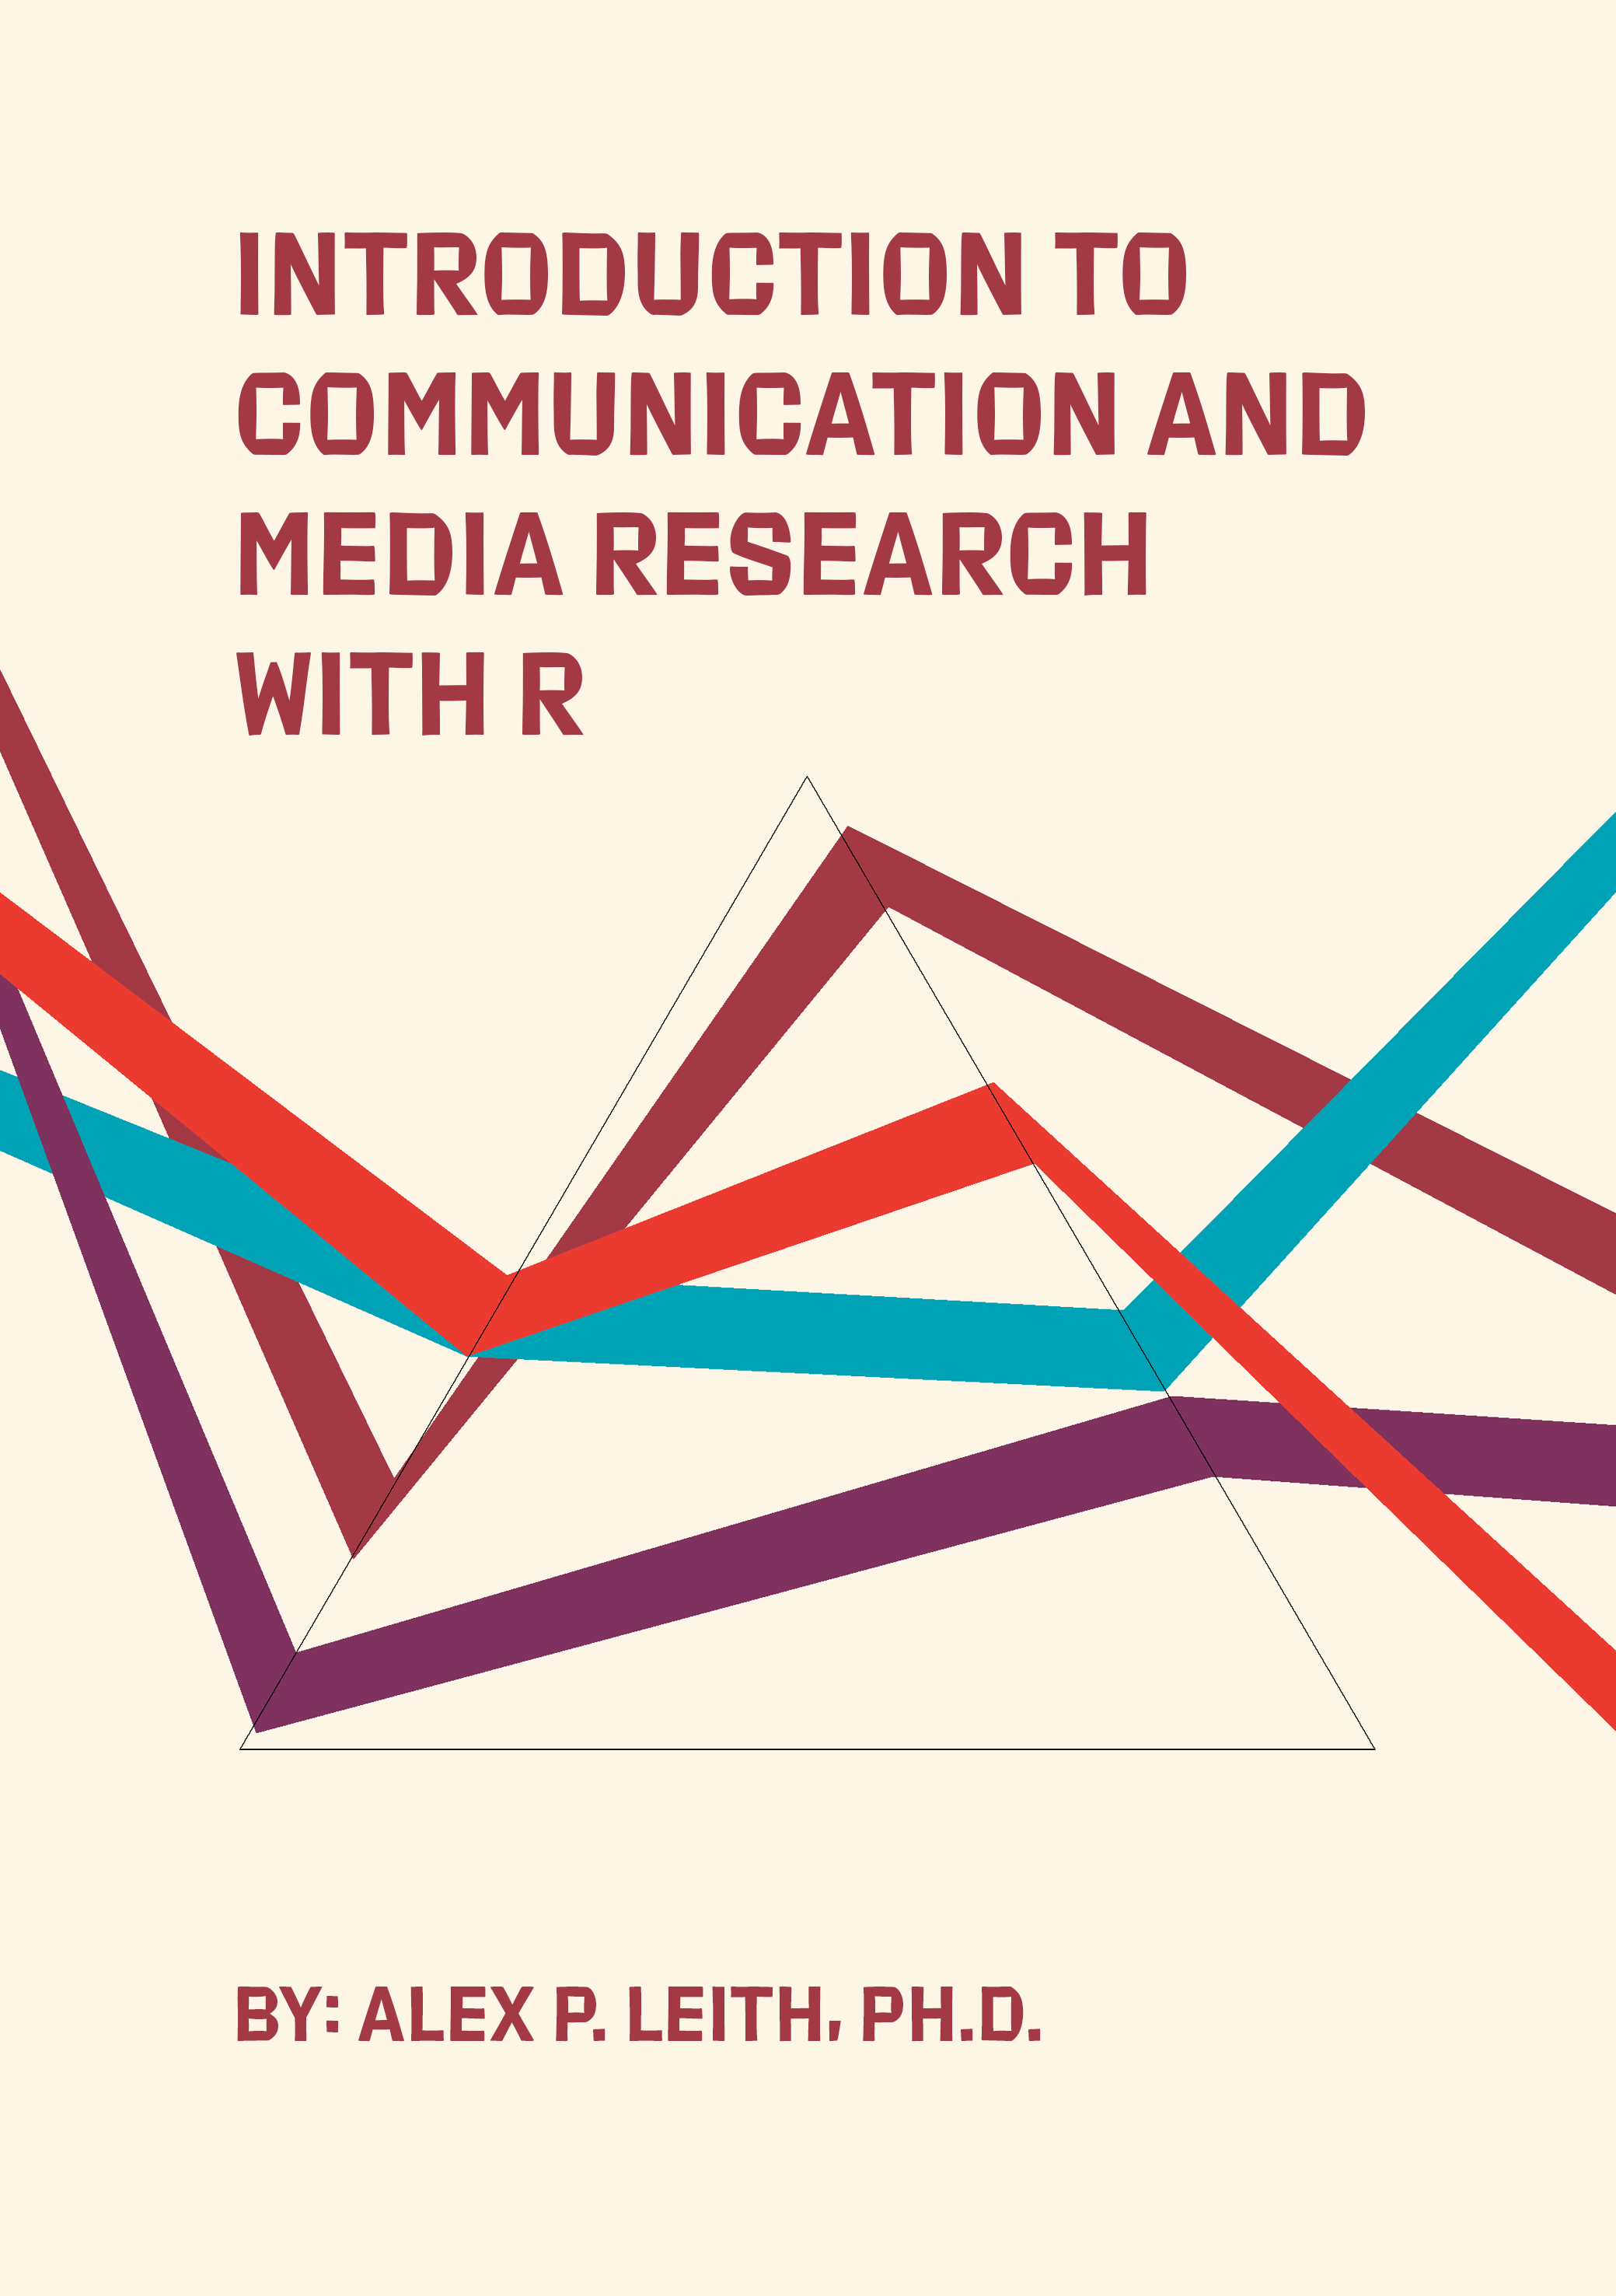
\includegraphics[width=0.5\textwidth,height=\textheight]{cover_2.png}}

This is an open-access textbook primarily created for my MC 451 course at Southern Illinois University Edwardsville (SIUE). I believe that it is important for our media and communication students to learn skills like R to better prepare them for the future of this industry.

Because coding is so frustrating to new learners, I hope this book will demystify the R language enough that they can use it to separate themselves in their future career. I also hope to make them more willing to tackle new complex systems on their own to continue to grow into the future of the communication and media fields.

This is a living document that will be continually adjusted according to feedback from other scholars and students. The current version of this book is a result of multiple semesters of teaching R to students in the Mass Communications department at SIUE, at both the undergraduate and graduate levels.

I would like to thank, and apologize to, each student that has trudged their way through this process with me. Your feedback has been greatly appreciated and instructive. I hope that each semester continues to become more approachable to students.

\hypertarget{introduction}{%
\chapter{Introduction}\label{introduction}}

Welcome to \emph{Introduction to Communication and Media Research with R}. I am Alex P. Leith, an Assistant Professor in the Mass Communications department at Southern Illinois University Edwardsville. While a doctoral student at Michigan State University, I fell in love with the flexibility of the R program for data collection, cleaning, analysis, and visualization. My intention with this book is to build an introductory research book for communication and media professionals that are tasked with research. For college students, this text is intended for individuals with either zero or limited research experience.

This book is also a practice in applying generative pre-trained transformers (GPT) in writing drafts. Namely, the first draft of this paper is a mix of human and AI writing. As I continue to work on this book, I will clean the text until limited traces of AI remain. I am using AI (e.g., Chat GPT, Google Bard) to identify future uses of these tools that still allow for individual work and learning opportunities. This book also borrows structure from existing research methods books. Images are pulled from royalty-free locations, such as Unsplash and Wikimedia.

Communication research systematically studies the processes, antecedents, and consequences of communication. It is a broad field encompassing various topics, from interpersonal to mass communication. Media research is the study of the effects of mass media on society, culture, and individuals. It encompasses a wide range of topics, including the impact of media on news consumption, political attitudes, and consumer behavior. Communication and media researchers use various methods to collect data, including surveys, interviews, focus groups, and experiments.

\hypertarget{research-ethics}{%
\section*{Research Ethics}\label{research-ethics}}
\addcontentsline{toc}{section}{Research Ethics}

Research ethics is the set of moral principles that guide the conduct of research. It is essential to ensure that research is conducted ethically to protect the rights and welfare of research participants, ensure the validity of research findings, and build public trust in research. Several ethical principles are relevant to research, including respect for persons, beneficence, and justice. In addition to these general ethical principles, there are also specific ethical guidelines for different types of research.

\hypertarget{research-papers}{%
\section*{Research Papers}\label{research-papers}}
\addcontentsline{toc}{section}{Research Papers}

An academic research paper is a piece of writing that presents the results of original research on a particular topic. It is typically written in a formal style and follows a specific format. Academic research papers are usually published in academic journals or presented at conferences. Research papers are discoverable through search engines available through academic libraries, publishers' websites, and search engines (e.g., Google Scholar).

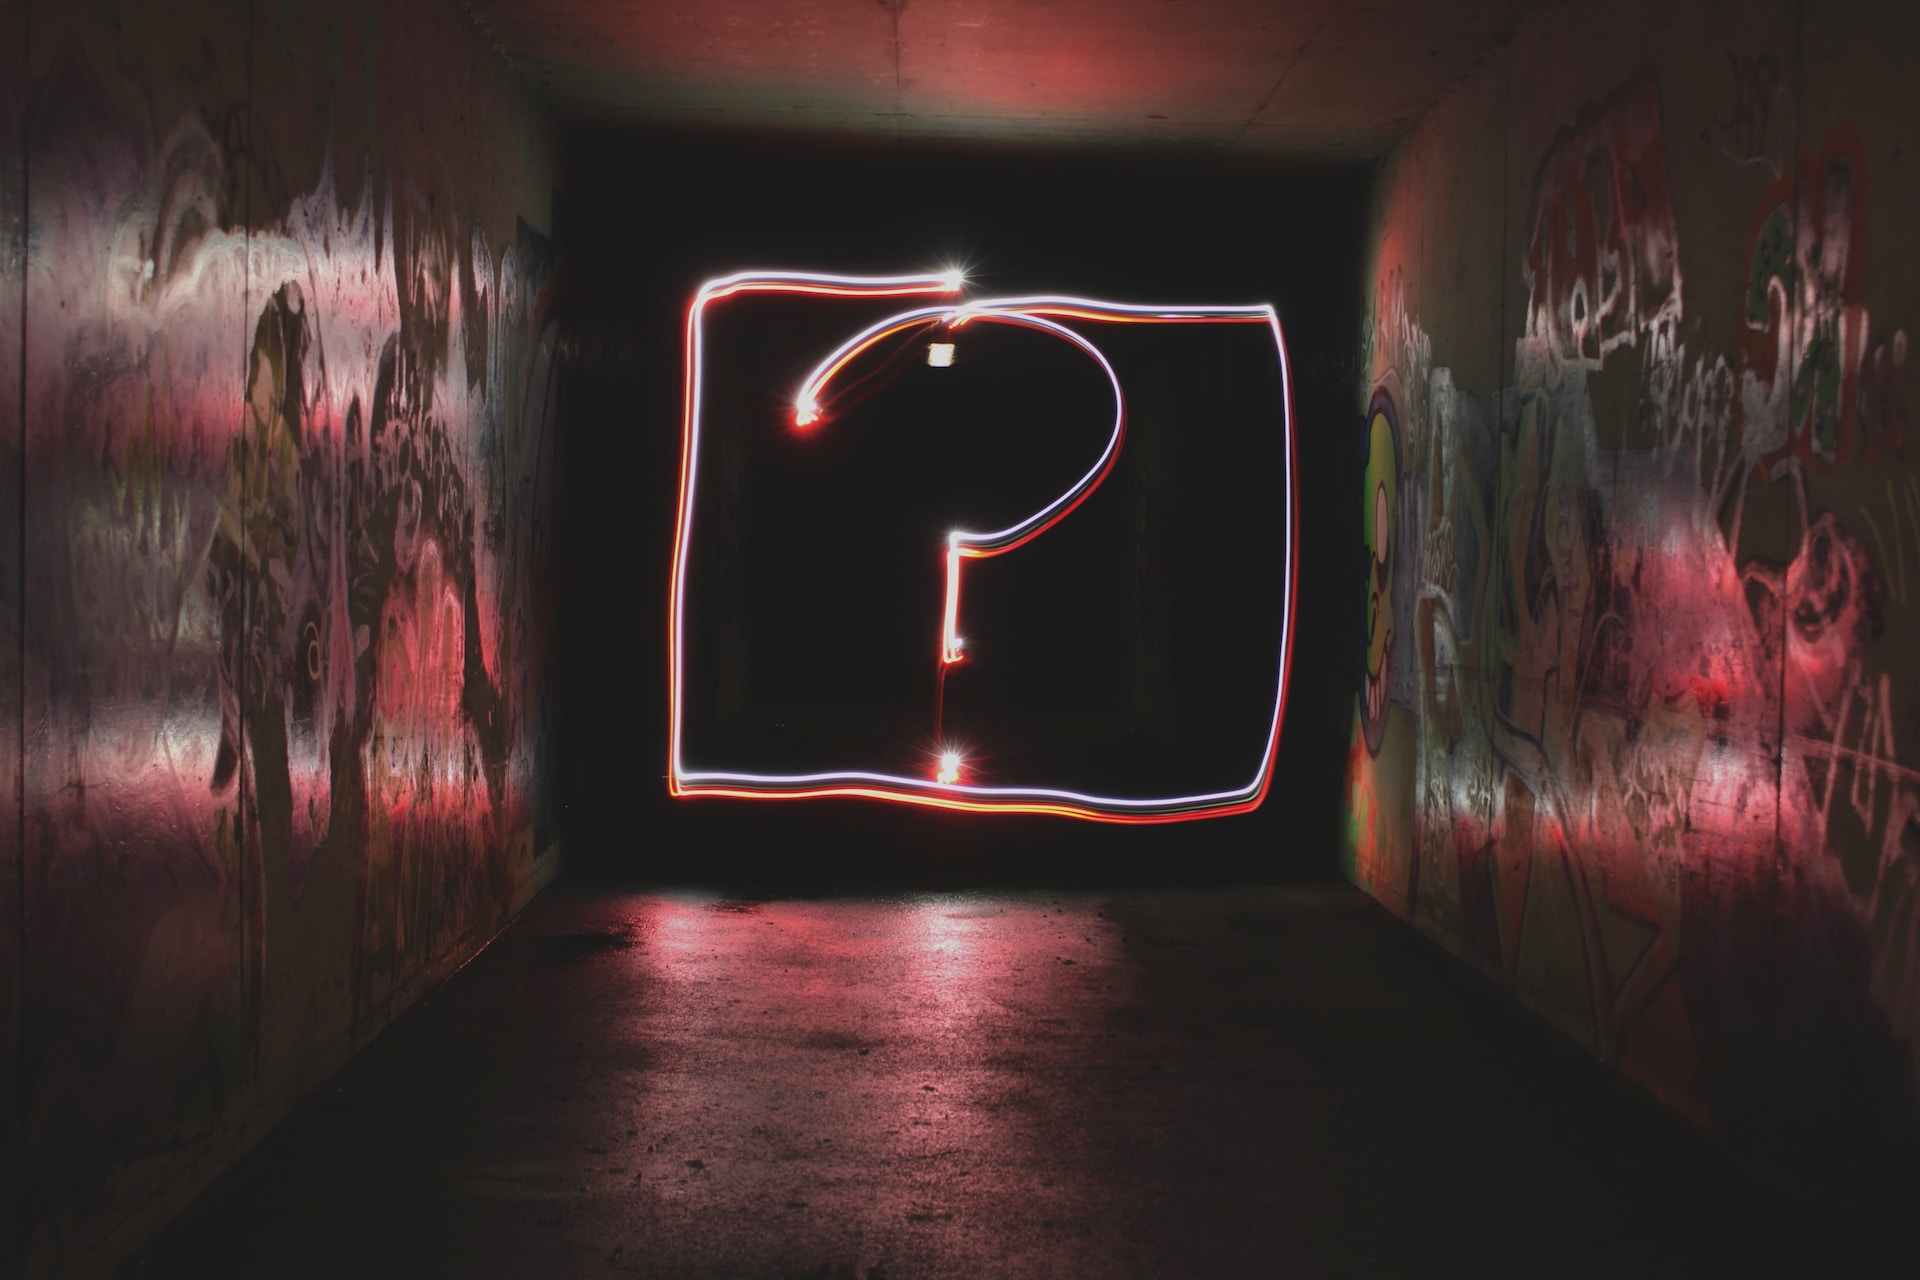
\includegraphics[width=1\textwidth,height=\textheight]{images/question_mark.jpg}

\hypertarget{communication-theories}{%
\section*{Communication Theories}\label{communication-theories}}
\addcontentsline{toc}{section}{Communication Theories}

Communication and media theories are a set of concepts and frameworks that help us understand how people communicate and how the media influences our lives. These theories can be used to analyze a wide range of communication phenomena, from interpersonal communication to mass media. Each theory offers a different perspective on how communication and the media work. By understanding these theories, we can better understand how people communicate and how the media influences our lives.

\hypertarget{interviews}{%
\section*{Interviews}\label{interviews}}
\addcontentsline{toc}{section}{Interviews}

Interviews are a research method in which the interviewer gathers information from the interviewee through open-ended questions and follow-up questions. The goal of a qualitative interview is to understand the interviewee's experiences, perspectives, and beliefs on a particular topic. Qualitative interviews are often used in social science research, but they can also be used in other fields, such as business, healthcare, and education. They are a valuable tool for gathering in-depth information that cannot be easily obtained through other methods, such as surveys or questionnaires. Interviews can be a valuable tool for researchers who want to understand the experiences, perspectives, and beliefs of people on a particular topic. However, it is important to note that qualitative interviews are not without their challenges. They can be time-consuming and expensive to conduct, and the data can be difficult to analyze. Additionally, the interviewer's own biases can influence the results of the interview.

\hypertarget{focus-groups}{%
\section*{Focus Groups}\label{focus-groups}}
\addcontentsline{toc}{section}{Focus Groups}

Focus groups are a research method in which a group of people are brought together to discuss a particular topic. The facilitator of the focus group asks open-ended questions and encourages the participants to share their thoughts and experiences. The goal of a focus group is to get a variety of perspectives on a particular topic and to understand how people interact with each other and with the topic. Focus groups can be a valuable tool for researchers who want to understand the perspectives of a group of people on a particular topic. However, it is important to note that qualitative focus groups are not without their challenges. They can be time-consuming and expensive to conduct, and the data can be difficult to analyze. Additionally, the facilitator's own biases can influence the results of the focus group.

\hypertarget{ethnography}{%
\section*{Ethnography}\label{ethnography}}
\addcontentsline{toc}{section}{Ethnography}

Ethnography is a research method that involves immersing the researcher in a particular culture or community to study its social interactions, behaviors, and beliefs. The researcher typically conducts participant observation, interviews, and document analysis to gather data. The goal of qualitative ethnography is to gain a deep understanding of the culture or community from the insider's perspective. Ethnography can be a valuable tool for researchers who want to understand the culture or community of a particular group of people. However, it is important to note that qualitative ethnography is not without its challenges. It can be time-consuming and expensive to conduct, and the researcher's own biases can influence the results of the study.

\hypertarget{qualitative-content-analysis}{%
\section*{Qualitative Content Analysis}\label{qualitative-content-analysis}}
\addcontentsline{toc}{section}{Qualitative Content Analysis}

Qualitative content analysis is a research method for the subjective interpretation of the content of text data through the systematic classification process of coding and identifying themes or patterns. The goal of qualitative content analysis is to understand the meaning of the text data by identifying patterns and themes. Qualitative content analysis can be a valuable tool for researchers who want to understand the meaning of text data. However, it is important to note that qualitative content analysis is not without its challenges. It can be time-consuming and labor-intensive to conduct, and the researcher's own biases can influence the results of the analysis.

\hypertarget{quantitative-content-analysis}{%
\section*{Quantitative Content Analysis}\label{quantitative-content-analysis}}
\addcontentsline{toc}{section}{Quantitative Content Analysis}

Quantitative content analysis is a research method for the objective, systematic, and quantitative description of the content of text data. The goal of quantitative content analysis is to quantify the presence of certain words, phrases, or concepts in a text and to analyze the relationships between these features. Quantitative content analysis can be a valuable tool for researchers who want to quantify the presence of certain words, phrases, or concepts in a text. However, it is important to note that quantitative content analysis is not without its challenges. It can be time-consuming and labor-intensive to conduct, and the researcher's own biases can still influence the results of the analysis.

\hypertarget{surveys}{%
\section*{Surveys}\label{surveys}}
\addcontentsline{toc}{section}{Surveys}

Surveys are a research method in which a researcher asks a set of questions to a group of people in order to collect numerical data. The data is then analyzed to answer research questions or test hypotheses. Surveys can be a valuable tool for researchers who want to collect data about a large group of people. However, it is important to note that quantitative surveys are not without their challenges. They can be time-consuming and expensive to conduct, and the respondents may not always answer the questions honestly or accurately.

\hypertarget{experiment}{%
\section*{Experiment}\label{experiment}}
\addcontentsline{toc}{section}{Experiment}

Experiment are research studies that use a scientific approach to test a hypothesis. The researcher manipulates one or more variables and then measures the effects of the manipulation on one or more other variables. Experiment can be a valuable tool for researchers who want to test a hypothesis and to determine the cause and effect relationship between two or more variables. However, it is important to note that quantitative experiments are not without their challenges. They can be time-consuming and expensive to conduct, and the results can be affected by the way the experiment is conducted.

\hypertarget{introduction-to-r}{%
\section*{Introduction to R}\label{introduction-to-r}}
\addcontentsline{toc}{section}{Introduction to R}

R is a programming language and software environment for statistical computing and graphics. It is a free and open-source software environment, making it available to everyone to use and modify. R is used by statisticians, data miners, and researchers in various fields. The program allows individuals to use code to expedite data cleaning and analysis tasks. Users are also provided with a range of options for data visualization.

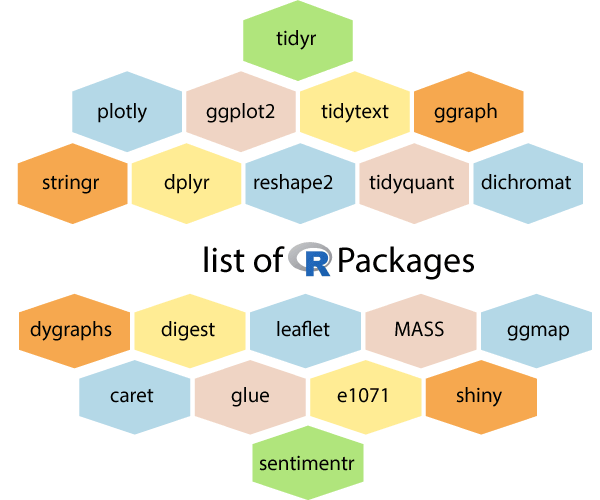
\includegraphics[width=1\textwidth,height=\textheight]{images/List-of-r-packages.png}

\hypertarget{working-with-data}{%
\section*{Working with Data}\label{working-with-data}}
\addcontentsline{toc}{section}{Working with Data}

Data is a collection of facts, figures, or observations that can be used to answer questions or test hypotheses. Data can be collected from various sources, including surveys, experiments, and observations. Once data has been collected, it needs to be prepared for analysis. This process typically involves cleaning the data, formatting the data, and transforming the data. Researchers can either use R for these stages or external programs (e.g., Excel).

\hypertarget{visuals}{%
\section*{Visuals}\label{visuals}}
\addcontentsline{toc}{section}{Visuals}

There are many different types of data visualization, each with strengths and weaknesses. Some of the most common types of data visualization include bar charts, scatter plots, images, or tables. The best kind of data visualization for a particular dataset depends on the specific research question and the study's goals. Choosing a data visualization that is easy to understand and accurately represents the data is essential.

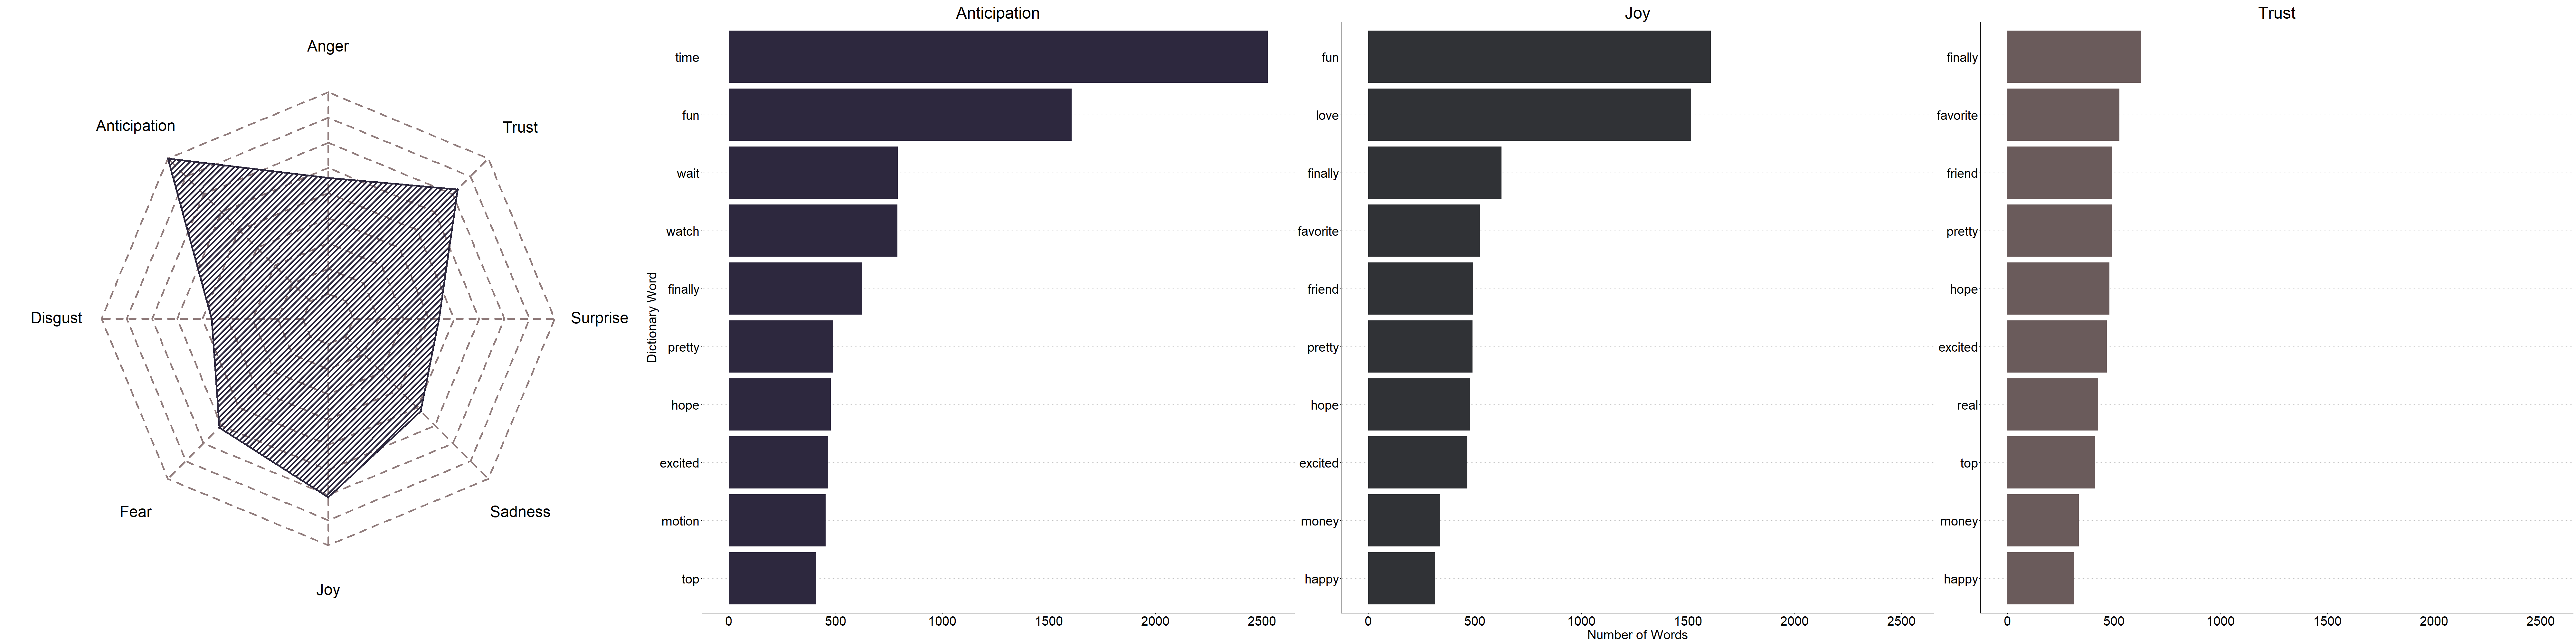
\includegraphics[width=1\textwidth,height=\textheight]{images/VR-Play-Emotion-MP.png}

\hypertarget{analyses}{%
\section*{Analyses}\label{analyses}}
\addcontentsline{toc}{section}{Analyses}

Data analysis is the process of inspecting, cleaning, transforming, and modeling data to discover useful information, inform conclusions, and support decision-making. Data analysis has multiple facets and approaches, encompassing diverse techniques under various names in different business, science, and social science domains. For our context, we are most interested in descriptive and inferential statistics. Descriptive statistics are used to summarize data and describe its main features. They can be used to calculate measures of central tendency (such as the mean, median, and mode) and measures of variation (such as the standard deviation). Inferential statistics are used to make inferences about a population based on a sample. They can be used to test hypotheses and estimate parameters. The best type of data analysis for a particular dataset will depend on the specific research question being asked and the goals of the study. Choosing a data analysis method that is appropriate for the data and will help answer the research question is vital.

\hypertarget{research-ethics-1}{%
\chapter{Research Ethics}\label{research-ethics-1}}

\hypertarget{history}{%
\section{History}\label{history}}

The history of research ethics in social science is a long and complex one. It has been shaped by a number of factors, including the development of new research methods, the rise of social movements, and public awareness of ethical violations.

In the early days of social science research, there were few formal ethical guidelines. Researchers often conducted their studies without any regard for the rights or welfare of their participants. This led to a number of high-profile ethical violations, such as the Tuskegee Syphilis Study and the Milgram Experiments.

These ethical violations led to a growing awareness of the need for ethical standards in social science research. In 1974, the U.S. Congress passed the National Research Act, which established the National Commission for the Protection of Human Subjects of Biomedical and Behavioral Research. This commission was tasked with developing ethical guidelines for social science research.

The commission's report, ``The Belmont Report,'' outlined three basic ethical principles for social science research: respect for persons, beneficence, and justice. These principles have been widely adopted by social scientists and have helped to shape the ethical landscape of social science research.

In recent years, there has been a growing emphasis on the need for cultural sensitivity in social science research. This is due in part to the increasing diversity of the world's population and the growing awareness of the ways in which culture can shape research findings.

As a result of these developments, the field of research ethics in social science is constantly evolving. New ethical challenges are emerging all the time, and researchers must be prepared to adapt their practices accordingly.

\hypertarget{key-events}{%
\subsection*{Key Events}\label{key-events}}
\addcontentsline{toc}{subsection}{Key Events}

\begin{itemize}
\tightlist
\item
  1949: The Nuremberg Code is adopted, outlining ethical principles for medical research involving human subjects.
\item
  1964: The Declaration of Helsinki is adopted, providing recommendations for biomedical research involving human subjects.
\item
  1974: The National Research Act is passed, establishing the National Commission for the Protection of Human Subjects of Biomedical and Behavioral Research.
\item
  1979: The Belmont Report is published, outlining three basic ethical principles for social science research: respect for persons, beneficence, and justice.
\item
  1991: The American Psychological Association adopts its first code of ethics for research with human participants.
\item
  2002: The National Bioethics Advisory Commission issues its report, ``Ethical and Policy Issues in Human Stem Cell Research,'' which discusses the ethical implications of stem cell research.
\item
  2013: The American Sociological Association adopts its first code of ethics for research with human participants.
\end{itemize}

\hypertarget{unethical-research}{%
\subsection*{Unethical Research}\label{unethical-research}}
\addcontentsline{toc}{subsection}{Unethical Research}

\hypertarget{the-tuskegee-syphilis-study}{%
\subsubsection*{The Tuskegee Syphilis Study}\label{the-tuskegee-syphilis-study}}
\addcontentsline{toc}{subsubsection}{The Tuskegee Syphilis Study}

This study, which ran from 1932 to 1972, involved 600 African American men who were infected with syphilis but not treated. The researchers observed the men's progression of the disease without providing them with treatment, even after penicillin became available. This study was unethical because it violated the men's right to informed consent and because it exposed them to unnecessary harm.

\hypertarget{the-milgram-experiments}{%
\subsubsection*{The Milgram Experiments}\label{the-milgram-experiments}}
\addcontentsline{toc}{subsubsection}{The Milgram Experiments}

\begin{longtable}[]{@{}
  >{\raggedright\arraybackslash}p{(\columnwidth - 2\tabcolsep) * \real{0.7778}}
  >{\raggedright\arraybackslash}p{(\columnwidth - 2\tabcolsep) * \real{0.2222}}@{}}
\toprule\noalign{}
\endhead
\bottomrule\noalign{}
\endlastfoot
These experiments, which were conducted by Stanley Milgram in the 1960s, investigated obedience to authority. In the experiments, participants were told to deliver electric shocks to another person, who was actually an actor. The shocks were fake, but the participants did not know this. Many of the participants continued to deliver shocks even when the actor was begging them to stop. This study was unethical because it caused psychological distress to the participants. & 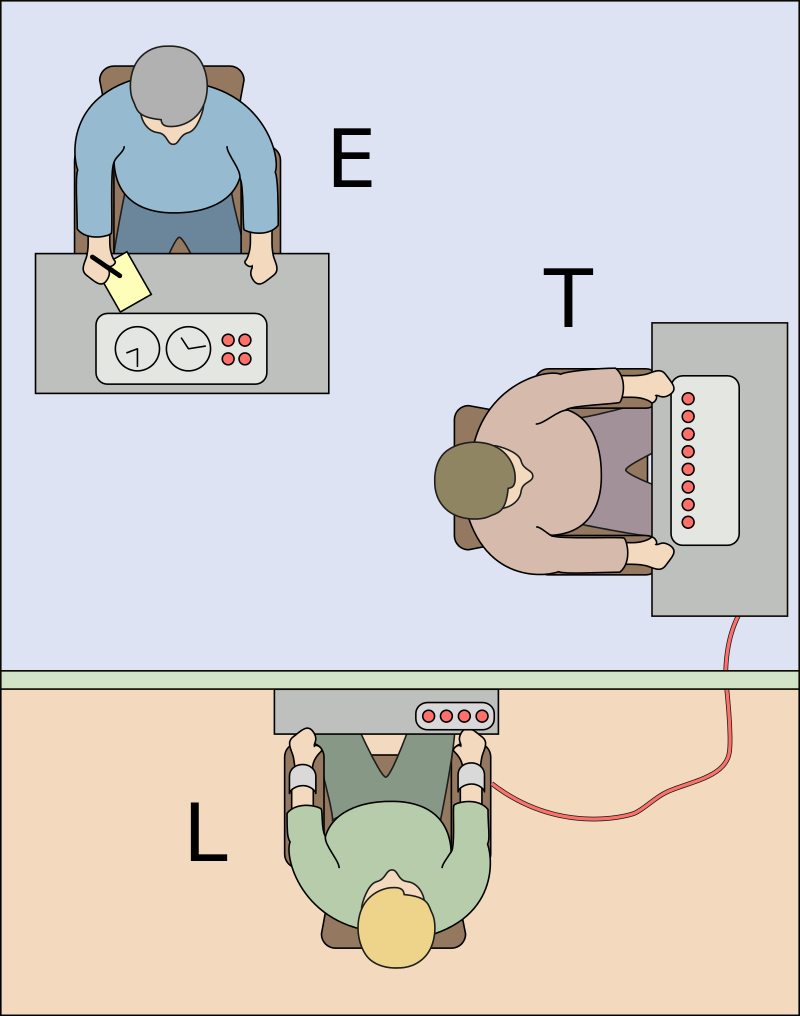
\includegraphics[width=1\textwidth,height=\textheight]{images/Milgram_experiment.png} \\
\end{longtable}

\hypertarget{the-stanford-prison-experiment}{%
\subsubsection*{The Stanford Prison Experiment}\label{the-stanford-prison-experiment}}
\addcontentsline{toc}{subsubsection}{The Stanford Prison Experiment}

\begin{longtable}[]{@{}
  >{\raggedright\arraybackslash}p{(\columnwidth - 2\tabcolsep) * \real{0.2222}}
  >{\raggedright\arraybackslash}p{(\columnwidth - 2\tabcolsep) * \real{0.7778}}@{}}
\toprule\noalign{}
\endhead
\bottomrule\noalign{}
\endlastfoot
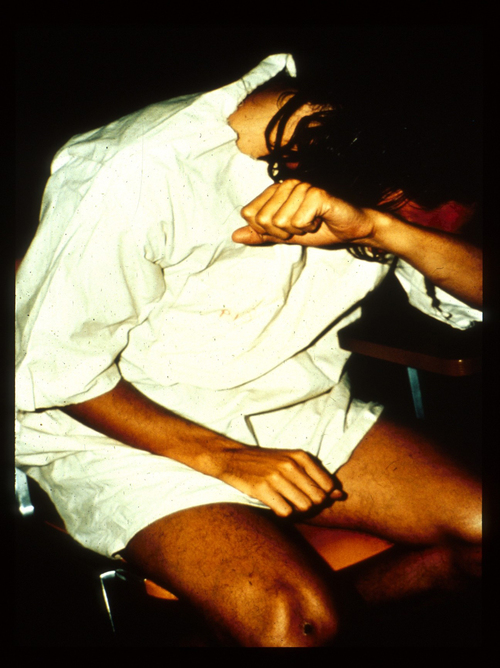
\includegraphics[width=1\textwidth,height=\textheight]{images/prisoner-breaks-down.png} & This experiment, which was conducted by Philip Zimbardo in 1971, simulated a prison environment. Participants were randomly assigned to be either guards or prisoners. The guards quickly began to abuse the prisoners, and the prisoners became increasingly submissive. This study was unethical because it created a stressful and potentially harmful environment for the participants. These are just a few examples of unethical applications of social science research. These studies have helped to raise awareness of the importance of ethical research practices, and they have led to the development of ethical guidelines for social science research. \\
\end{longtable}

\hypertarget{key-components}{%
\section*{Key Components}\label{key-components}}
\addcontentsline{toc}{section}{Key Components}

\emph{The key components of research ethics}

\hypertarget{informed-consent}{%
\subsection*{Informed Consent}\label{informed-consent}}
\addcontentsline{toc}{subsection}{Informed Consent}

Participants must be given adequate information about the research in order to make an informed decision about whether or not to participate. This information should include title of project, names of researchers, contact info for researchers, purpose of study, procedures, risks \& benefits, and anonymity, voluntary participation.

\hypertarget{confidentiality}{%
\subsection*{Confidentiality}\label{confidentiality}}
\addcontentsline{toc}{subsection}{Confidentiality}

The privacy of participants must be protected. This means that researchers must not share personal information about participants without their consent.

\hypertarget{debriefing}{%
\subsection*{Debriefing}\label{debriefing}}
\addcontentsline{toc}{subsection}{Debriefing}

Participants must be debriefed after the research is completed. This means that they must be given more information about the research, including any deception that was used. Participants also have the right to ask questions and to have their concerns addressed.

\hypertarget{avoidance-of-harm}{%
\subsection*{Avoidance of Harm}\label{avoidance-of-harm}}
\addcontentsline{toc}{subsection}{Avoidance of Harm}

Participants must not be harmed by the research. This means that researchers must take steps to minimize the risks of harm to participants.

\hypertarget{justice}{%
\subsection*{Justice}\label{justice}}
\addcontentsline{toc}{subsection}{Justice}

The benefits and burdens of research must be distributed fairly. This means that researchers must ensure that all participants have an equal opportunity to benefit from the research, and that no one group is disproportionately burdened by the research.

\hypertarget{ethical-considerations}{%
\section*{Ethical Considerations}\label{ethical-considerations}}
\addcontentsline{toc}{section}{Ethical Considerations}

In addition to these key components, there are a number of other ethical considerations that researchers must take into account. Researchers must carefully consider all of these ethical issues when designing and conducting research. By following ethical principles, researchers can help to ensure that their research is conducted in an ethical manner and that the rights and welfare of participants are protected.

\hypertarget{deception}{%
\subsection*{Deception}\label{deception}}
\addcontentsline{toc}{subsection}{Deception}

Deception can be used in research to prevent participants from guessing the purpose of the study. However, deception can also harm participants by making them feel misled or violated.

\hypertarget{risks-to-participants}{%
\subsection*{Risks to Participants}\label{risks-to-participants}}
\addcontentsline{toc}{subsection}{Risks to Participants}

Some research involves risks to participants, such as physical or psychological harm. These risks must be weighed against the potential benefits of the research before participants can consent to participate.

\hypertarget{vulnerable-populations}{%
\subsection*{Vulnerable Populations}\label{vulnerable-populations}}
\addcontentsline{toc}{subsection}{Vulnerable Populations}

Some populations are more vulnerable to harm from research, such as children, prisoners, and people with disabilities. These populations require special protections in research.

\hypertarget{intellectual-property}{%
\subsection*{Intellectual Property}\label{intellectual-property}}
\addcontentsline{toc}{subsection}{Intellectual Property}

Researchers must be careful not to violate the intellectual property rights of others, such as by publishing data without permission or using copyrighted materials without permission.

\hypertarget{current-ethical-challenges-in-social-science-research}{%
\section{Current Ethical Challenges in Social Science Research}\label{current-ethical-challenges-in-social-science-research}}

The use of new technologies, such as social media and big data, raises new ethical challenges. The need for cultural sensitivity in social science research is becoming increasingly important. The tension between the need for confidentiality and the need to share research findings with the public is a challenge that researchers must grapple with. The increasing commercialization of social science research raises ethical concerns about the potential for conflicts of interest.

\hypertarget{institutional-review-board}{%
\section{Institutional Review Board}\label{institutional-review-board}}

\hypertarget{history-of-the-institutional-review-board}{%
\subsection*{History of the Institutional Review Board}\label{history-of-the-institutional-review-board}}
\addcontentsline{toc}{subsection}{History of the Institutional Review Board}

The Institutional Review Board (IRB) is a committee that reviews research involving human subjects to ensure that the research is conducted ethically. IRBs are required by law in the United States and in many other countries.

The history of IRBs can be traced back to the Nuremberg Code, which was adopted in 1949 in response to the atrocities committed by Nazi doctors during World War II. The Nuremberg Code established basic ethical principles for medical research involving human subjects, including the need for informed consent and the avoidance of unnecessary harm.

In 1964, the Declaration of Helsinki was adopted, providing additional guidance on ethical research practices. The Declaration of Helsinki was revised in 2013 to reflect the changing landscape of biomedical research.

In the United States, the National Research Act of 1974 established the National Commission for the Protection of Human Subjects of Biomedical and Behavioral Research. The commission was tasked with developing ethical guidelines for research involving human subjects. The commission's report, ``The Belmont Report,'' outlined three basic ethical principles for research involving human subjects: respect for persons, beneficence, and justice.

The Belmont Report has been widely adopted by IRBs and has helped to shape the ethical landscape of research involving human subjects. IRBs are responsible for ensuring that research involving human subjects is conducted in accordance with the ethical principles outlined in the Belmont Report.

\hypertarget{purpose-of-the-institutional-review-board}{%
\subsection*{Purpose of the Institutional Review Board}\label{purpose-of-the-institutional-review-board}}
\addcontentsline{toc}{subsection}{Purpose of the Institutional Review Board}

The purpose of the IRB is to protect the rights and welfare of human subjects involved in research. IRBs do this by reviewing research proposals to ensure that they meet ethical standards. IRBs play an important role in protecting the rights and welfare of human subjects involved in research. By reviewing research proposals and ensuring that research is conducted in accordance with ethical standards, IRBs help to ensure that research is conducted in a responsible and ethical manner.

IRBs review research proposals for a number of factors, including:

\begin{itemize}
\tightlist
\item
  The risks and benefits of the research
\item
  The informed consent process
\item
  The protection of confidentiality
\item
  The selection of research subjects
\end{itemize}

If an IRB finds that a research proposal does not meet ethical standards, the proposal may be modified or rejected.

\hypertarget{levels-of-risk}{%
\subsection*{Levels of Risk}\label{levels-of-risk}}
\addcontentsline{toc}{subsection}{Levels of Risk}

The three levels of risk for IRB are:

\hypertarget{exempt}{%
\subsubsection*{Exempt}\label{exempt}}
\addcontentsline{toc}{subsubsection}{Exempt}

Studies that meet the criteria for exemption from IRB review do not pose more than minimal risk to participants. Examples of exempt studies include:

\begin{itemize}
\item
  Research using existing data or records that cannot be linked back to individual participants.
\item
  Research involving surveys or interviews that do not ask about sensitive topics.
\item
  Research involving the observation of public behavior.
\end{itemize}

\hypertarget{expedited}{%
\subsubsection*{Expedited}\label{expedited}}
\addcontentsline{toc}{subsubsection}{Expedited}

Studies that involve no more than minimal risk to participants and meet the criteria for expedited review may be reviewed by a single IRB reviewer or a small committee of reviewers. Examples of expedited studies include:

\begin{itemize}
\item
  Research involving the use of noninvasive procedures, such as blood pressure checks or physical exams.
\item
  Research involving the collection of non-sensitive data, such as demographic information or data about food choices.
\item
  Research involving the use of existing data or records that can be linked back to individual participants, but only if the data is de-identified.
\end{itemize}

\hypertarget{full}{%
\subsubsection*{Full}\label{full}}
\addcontentsline{toc}{subsubsection}{Full}

Studies that involve more than minimal risk to participants or do not meet the criteria for exempt or expedited review must be reviewed by the full IRB. Examples of full board studies include:

\begin{itemize}
\item
  Research involving the use of invasive procedures, such as surgery or blood draws.
\item
  Research involving the collection of sensitive data, such as information about mental health or sexual behavior.
\item
  Research involving the use of deception or coercion.
\end{itemize}

\hypertarget{references}{%
\section{References}\label{references}}

American Psychological Association (2017). Ethical principles of psychologists and code of conduct. Retrieved from \url{https://www.apa.org/ethics/code/}

Brandt, A. M. (1978). Racism and research: The case of the Tuskegee Syphilis Study. Daedalus, 107(2), 17-41.

Milgram, S. (1974). Obedience to authority: An experimental view. New York, NY: Harper \& Row.

National Commission for the Protection of Human Subjects of Biomedical and Behavioral Research. (1979). The Belmont Report: Ethical principles and guidelines for the protection of human subjects of research. Washington, DC: U.S. Government Printing Office.

National Institutes of Health (2019). Protecting human subjects. Retrieved from \url{https://humansubjects.nih.gov/}

Office for Human Research Protections (2022). Protecting human subjects. Retrieved from \url{https://www.hhs.gov/ohrp/index.html}

U.S. Department of Health and Human Services. (2018). Protection of human subjects. Retrieved from \url{https://www.hhs.gov/ohrp/humansubjects/index.html}

Zimbardo, P. G. (2007). The Lucifer effect: Understanding how good people turn evil. New York, NY: Random House.

\hypertarget{research-papers-1}{%
\chapter{Research Papers}\label{research-papers-1}}

\hypertarget{how-to-find-research-papers}{%
\section{How to Find Research Papers}\label{how-to-find-research-papers}}

There are many ways to find research papers, both paid and free. Here are a few popular methods:

\hypertarget{search-location}{%
\subsection*{Search Location}\label{search-location}}
\addcontentsline{toc}{subsection}{Search Location}

\hypertarget{use-a-specialized-search-engine.}{%
\subsubsection*{Use a specialized search engine.}\label{use-a-specialized-search-engine.}}
\addcontentsline{toc}{subsubsection}{Use a specialized search engine.}

There are many specialized search engines that are designed for finding research papers. Some of the most popular ones include Google Scholar, Microsoft Academic, and Scopus. These search engines index a large number of academic journals and repositories, making it easy to find relevant papers.

\hypertarget{check-your-university-library.}{%
\subsubsection*{Check your university library.}\label{check-your-university-library.}}
\addcontentsline{toc}{subsubsection}{Check your university library.}

If you are a student or faculty member at a university, you likely have access to a library that subscribes to a variety of academic journals. You can use the library's catalog to search for research papers by title, author, or keyword.

\hypertarget{search-for-preprints.}{%
\subsubsection*{Search for preprints.}\label{search-for-preprints.}}
\addcontentsline{toc}{subsubsection}{Search for preprints.}

Preprints are research papers that have been submitted to a journal but have not yet been peer-reviewed and published. Preprints are often available for free on websites like arXiv and bioRxiv.

\hypertarget{use-social-media.}{%
\subsubsection*{Use social media.}\label{use-social-media.}}
\addcontentsline{toc}{subsubsection}{Use social media.}

Many researchers use social media to share their work, including research papers. You can follow researchers in your field on Twitter, LinkedIn, and Facebook to see if they have shared any papers that you might be interested in.

\hypertarget{contact-experts-in-your-field.}{%
\subsubsection*{Contact experts in your field.}\label{contact-experts-in-your-field.}}
\addcontentsline{toc}{subsubsection}{Contact experts in your field.}

If you are struggling to find research papers on a particular topic, you can contact experts in your field and ask for their recommendations. Experts are often happy to share their research with others.

\hypertarget{tips-for-searching}{%
\subsection*{Tips for Searching}\label{tips-for-searching}}
\addcontentsline{toc}{subsection}{Tips for Searching}

Here are some additional tips for finding research papers:

\hypertarget{use-specific-keywords.}{%
\subsubsection*{Use specific keywords.}\label{use-specific-keywords.}}
\addcontentsline{toc}{subsubsection}{Use specific keywords.}

The more specific your keywords are, the more likely you are to find relevant papers. For example, instead of searching for ``artificial intelligence,'' you could search for ``deep learning for natural language processing.''

\hypertarget{use-advanced-search-features.}{%
\subsubsection*{Use advanced search features.}\label{use-advanced-search-features.}}
\addcontentsline{toc}{subsubsection}{Use advanced search features.}

Many search engines have advanced search features that allow you to narrow down your results. For example, you can search for papers that have been published in a particular journal or that have been cited a certain number of times.

\hypertarget{use-multiple-search-engines.}{%
\subsubsection*{Use multiple search engines.}\label{use-multiple-search-engines.}}
\addcontentsline{toc}{subsubsection}{Use multiple search engines.}

No single search engine indexes all of the world's research papers. By using multiple search engines, you can increase your chances of finding the papers you are looking for.

\hypertarget{be-patient.}{%
\subsubsection*{Be patient.}\label{be-patient.}}
\addcontentsline{toc}{subsubsection}{Be patient.}

It can take some time to find the right research papers. Don't give up if you don't find what you are looking for right away. Keep searching and you will eventually find the papers you need.

I hope this helps!

\hypertarget{how-to-read-research-papers}{%
\section{How to Read Research Papers}\label{how-to-read-research-papers}}

\hypertarget{common-approaches}{%
\subsection*{Common Approaches}\label{common-approaches}}
\addcontentsline{toc}{subsection}{Common Approaches}

There are many different approaches to reading a research paper, but these are some of the most effective ones.

\hypertarget{the-three-pass-approach.}{%
\subsubsection*{The three-pass approach.}\label{the-three-pass-approach.}}
\addcontentsline{toc}{subsubsection}{The three-pass approach.}

This approach involves reading the paper three times, each time with a different goal in mind. The first pass is a quick skim to get an overview of the paper. The second pass is a more detailed read, focusing on the key points and arguments. The third pass is a critical read, where you evaluate the paper's methods, results, and conclusions.

\hypertarget{the-question-based-approach.}{%
\subsubsection*{The question-based approach.}\label{the-question-based-approach.}}
\addcontentsline{toc}{subsubsection}{The question-based approach.}

This approach involves reading the paper with a specific set of questions in mind. This can help you stay focused and avoid getting bogged down in the details. Some good questions to ask include:

\begin{itemize}
\item
  What is the main question that the paper is trying to answer?
\item
  What are the key findings of the paper?
\item
  How did the authors conduct their research?
\item
  Are the results of the research reliable?
\item
  What are the implications of the research?
\end{itemize}

\hypertarget{the-active-reading-approach.}{%
\subsubsection*{The active reading approach.}\label{the-active-reading-approach.}}
\addcontentsline{toc}{subsubsection}{The active reading approach.}

This approach involves taking notes, highlighting important passages, and asking questions as you read. This can help you engage with the material and make sure that you understand it.

\hypertarget{the-collaborative-reading-approach.}{%
\subsubsection*{The collaborative reading approach.}\label{the-collaborative-reading-approach.}}
\addcontentsline{toc}{subsubsection}{The collaborative reading approach.}

This approach involves reading the paper with a partner or group of people. This can be helpful for getting different perspectives on the paper and for identifying areas where you need clarification.

No matter which approach you choose, it is important to take your time and read the paper carefully. Research papers can be dense and challenging, but they can also be very rewarding. By taking the time to read them carefully, you can learn a lot about your field and contribute to the advancement of knowledge.

\hypertarget{additional-tips}{%
\subsection*{Additional Tips}\label{additional-tips}}
\addcontentsline{toc}{subsection}{Additional Tips}

Here are some additional tips for reading research papers:

\hypertarget{set-a-goal-for-yourself.}{%
\subsubsection*{Set a goal for yourself.}\label{set-a-goal-for-yourself.}}
\addcontentsline{toc}{subsubsection}{Set a goal for yourself.}

What do you hope to learn from reading the paper?

\hypertarget{read-actively.}{%
\subsubsection*{Read actively.}\label{read-actively.}}
\addcontentsline{toc}{subsubsection}{Read actively.}

Take notes, highlight important passages, and ask questions.

\hypertarget{dont-be-afraid-to-take-breaks.}{%
\subsubsection*{Don't be afraid to take breaks.}\label{dont-be-afraid-to-take-breaks.}}
\addcontentsline{toc}{subsubsection}{Don't be afraid to take breaks.}

If you get stuck, take a break and come back to it later.

\hypertarget{consult-with-experts.}{%
\subsubsection*{Consult with experts.}\label{consult-with-experts.}}
\addcontentsline{toc}{subsubsection}{Consult with experts.}

If you don't understand something, ask an expert for help.

\hypertarget{be-critical.}{%
\subsubsection*{Be critical.}\label{be-critical.}}
\addcontentsline{toc}{subsubsection}{Be critical.}

Evaluate the paper's methods, results, and conclusions.

\hypertarget{take-notes.}{%
\subsubsection*{Take notes.}\label{take-notes.}}
\addcontentsline{toc}{subsubsection}{Take notes.}

This will help you remember what you learned and refer back to the paper later.

\hypertarget{summarize-the-paper.}{%
\subsubsection*{Summarize the paper.}\label{summarize-the-paper.}}
\addcontentsline{toc}{subsubsection}{Summarize the paper.}

This will help you solidify your understanding of the paper.

\hypertarget{discuss-the-paper-with-others.}{%
\subsubsection*{Discuss the paper with others.}\label{discuss-the-paper-with-others.}}
\addcontentsline{toc}{subsubsection}{Discuss the paper with others.}

This will help you gain different perspectives on the paper.

\hypertarget{how-to-write-research-papers}{%
\section{How to Write Research Papers}\label{how-to-write-research-papers}}

\hypertarget{common-approaches-1}{%
\subsection*{Common Approaches}\label{common-approaches-1}}
\addcontentsline{toc}{subsection}{Common Approaches}

There are many different approaches to writing a research paper, but some of the most effective ones include:

\hypertarget{choose-an-interesting-topic-you-know.}{%
\subsubsection*{Choose an interesting topic you know.}\label{choose-an-interesting-topic-you-know.}}
\addcontentsline{toc}{subsubsection}{Choose an interesting topic you know.}

This will make the research process more enjoyable and you will be more likely to produce a high-quality paper.

\hypertarget{do-your-research-thoroughly.}{%
\subsubsection*{Do your research thoroughly.}\label{do-your-research-thoroughly.}}
\addcontentsline{toc}{subsubsection}{Do your research thoroughly.}

Read as many relevant research papers as you can and take good notes. This will help you to develop a strong understanding of the topic and to form your own arguments.

\hypertarget{write-a-clear-and-concise-thesis-statement.}{%
\subsubsection*{Write a clear and concise thesis statement.}\label{write-a-clear-and-concise-thesis-statement.}}
\addcontentsline{toc}{subsubsection}{Write a clear and concise thesis statement.}

This should be a one-sentence statement that summarizes the main argument of your paper.

\hypertarget{organize-your-paper-carefully.}{%
\subsubsection*{Organize your paper carefully.}\label{organize-your-paper-carefully.}}
\addcontentsline{toc}{subsubsection}{Organize your paper carefully.}

Use an outline to help you structure your paper and to make sure that it flows smoothly.

\hypertarget{write-in-a-clear-and-concise-style.}{%
\subsubsection*{Write in a clear and concise style.}\label{write-in-a-clear-and-concise-style.}}
\addcontentsline{toc}{subsubsection}{Write in a clear and concise style.}

Avoid using jargon and technical terms that your audience may not understand.

\hypertarget{use-evidence-to-support-your-arguments.}{%
\subsubsection*{Use evidence to support your arguments.}\label{use-evidence-to-support-your-arguments.}}
\addcontentsline{toc}{subsubsection}{Use evidence to support your arguments.}

Cite your sources properly and use quotes, paraphrases, and summaries to support your claims.

\hypertarget{proofread-your-paper-carefully.}{%
\subsubsection*{Proofread your paper carefully.}\label{proofread-your-paper-carefully.}}
\addcontentsline{toc}{subsubsection}{Proofread your paper carefully.}

Make sure that there are no errors in grammar, spelling, or punctuation.

\hypertarget{additional-tips-1}{%
\subsection*{Additional Tips}\label{additional-tips-1}}
\addcontentsline{toc}{subsection}{Additional Tips}

Here are some additional tips for writing a research paper:

\hypertarget{start-early.}{%
\subsubsection*{Start early.}\label{start-early.}}
\addcontentsline{toc}{subsubsection}{Start early.}

Don't wait until the last minute to start writing your paper. This will give you enough time to do your research thoroughly and to write a well-organized paper.

\hypertarget{get-feedback-from-others.}{%
\subsubsection*{Get feedback from others.}\label{get-feedback-from-others.}}
\addcontentsline{toc}{subsubsection}{Get feedback from others.}

Ask a friend, family member, or professor to read your paper and give you feedback. This can help you to identify areas where your paper can be improved.

\hypertarget{dont-be-afraid-to-revise.}{%
\subsubsection*{Don't be afraid to revise.}\label{dont-be-afraid-to-revise.}}
\addcontentsline{toc}{subsubsection}{Don't be afraid to revise.}

It is important to revise your paper multiple times before you submit it. This will help you to improve your writing style and to make sure that your paper is error-free.

\hypertarget{take-breaks.}{%
\subsubsection*{Take breaks.}\label{take-breaks.}}
\addcontentsline{toc}{subsubsection}{Take breaks.}

Don't try to write your paper in one sitting. Take breaks to clear your head and to come back to it with fresh eyes.

\hypertarget{academic-examples}{%
\subsection*{Academic Examples}\label{academic-examples}}
\addcontentsline{toc}{subsection}{Academic Examples}

\hypertarget{industry-examples}{%
\subsection*{Industry Examples}\label{industry-examples}}
\addcontentsline{toc}{subsection}{Industry Examples}

\hypertarget{how-to-cite-research-papers}{%
\section{How to Cite Research Papers}\label{how-to-cite-research-papers}}

\hypertarget{two-types-in-apa}{%
\subsection*{Two Types in APA}\label{two-types-in-apa}}
\addcontentsline{toc}{subsection}{Two Types in APA}

The American Psychological Association (APA) style is a popular format for citing sources in academic papers. Here are the basic steps on how to cite research papers using APA:

\hypertarget{in-text-citations.}{%
\subsubsection*{In-text citations.}\label{in-text-citations.}}
\addcontentsline{toc}{subsubsection}{In-text citations.}

In-text citations are used to give credit to the sources you used in your paper. They are placed in parentheses after the information you are citing, and they include the author's last name, the year of publication, and the page number(s) where the information can be found. For example, if you are citing a quote from a book by John Smith, published in 2023, on page 100, your in-text citation would look like this: (Smith, 2023, p.~100).

\hypertarget{reference-list.}{%
\subsubsection*{Reference list.}\label{reference-list.}}
\addcontentsline{toc}{subsubsection}{Reference list.}

The reference list is a list of all the sources you used in your paper. It is placed at the end of your paper, and it is organized alphabetically by the author's last name. Each entry in the reference list includes the author's name, the year of publication, the title of the source, the publication information, and any other relevant information. For example, the reference list entry for the book by John Smith would look like this:

\begin{quote}
Smith, J. (2023). \emph{The Psychology of Learning}. New York, NY: Oxford University Press.
\end{quote}

Here is the template for each of the typical types of APA citations. Please review the APA website or Purdue's Writing Lab (OWL) for additional help with APA 7th.

\hypertarget{book.}{%
\paragraph*{Book.}\label{book.}}
\addcontentsline{toc}{paragraph}{Book.}

Author, A. A. (Year of publication). \emph{Title of work: Capital letter also for subtitle}. Publisher Name. DOI (if available)

\hypertarget{chapter-in-an-edited-book.}{%
\paragraph*{Chapter in an Edited Book.}\label{chapter-in-an-edited-book.}}
\addcontentsline{toc}{paragraph}{Chapter in an Edited Book.}

Author, A. A., \& Author, B. B. (Year of publication). Title of chapter. In E. E. Editor \& F. F. Editor (Eds.), \emph{Title of work: Capital letter also for subtitle} (pp.~pages of chapter). Publisher.~DOI (if available)

\hypertarget{journal-article.}{%
\paragraph*{Journal article.}\label{journal-article.}}
\addcontentsline{toc}{paragraph}{Journal article.}

Lastname, F. M., \& Lastname, F. M. (Year). Title of article. \emph{Title of Periodical, Vol.(}Issue), page numbers. DOI

\hypertarget{website.}{%
\paragraph*{Website.}\label{website.}}
\addcontentsline{toc}{paragraph}{Website.}

Lastname, F. M. (Year, Month Date). \emph{Title of page}. Site name. URL

\hypertarget{dissertation.}{%
\paragraph*{Dissertation.}\label{dissertation.}}
\addcontentsline{toc}{paragraph}{Dissertation.}

Lastname, F. M. (Year). \emph{Title of dissertation/thesis} (Publication No.) {[}Doctoral dissertation/Master's thesis, Name of Institution Awarding the Degree{]}. Database or Archive Name.

\hypertarget{report-by-government-agency.}{%
\paragraph*{Report by Government Agency.}\label{report-by-government-agency.}}
\addcontentsline{toc}{paragraph}{Report by Government Agency.}

Organization Name. (Year). \emph{Title of report.} URL

\hypertarget{report-by-individual.}{%
\paragraph*{Report by Individual.}\label{report-by-individual.}}
\addcontentsline{toc}{paragraph}{Report by Individual.}

Lastname, F. M., \& Lastname, F. M. (Year). \emph{Title of report}. Organization Name. URL

\hypertarget{tweet.}{%
\paragraph*{Tweet.}\label{tweet.}}
\addcontentsline{toc}{paragraph}{Tweet.}

Lastname, F. M. or Name of Group {[}@username{]}. (Year, Month Date).~\emph{Content of the post up to the first 20 words}{[}Tweet{]}. Site Name. URL

\hypertarget{additional-tips-2}{%
\subsection*{Additional Tips}\label{additional-tips-2}}
\addcontentsline{toc}{subsection}{Additional Tips}

Here are some additional tips for citing research papers using APA:

\hypertarget{use-a-consistent-style.}{%
\subsubsection*{Use a consistent style.}\label{use-a-consistent-style.}}
\addcontentsline{toc}{subsubsection}{Use a consistent style.}

This will help to make your paper look professional and polished.

\hypertarget{carefully-check-your-citations.}{%
\subsubsection*{Carefully check your citations.}\label{carefully-check-your-citations.}}
\addcontentsline{toc}{subsubsection}{Carefully check your citations.}

Make sure that you have included all of the necessary information, and that you have formatted your citations correctly.

\hypertarget{use-a-citation-management-tool.}{%
\subsubsection*{Use a citation management tool.}\label{use-a-citation-management-tool.}}
\addcontentsline{toc}{subsubsection}{Use a citation management tool.}

This can save you time and help to ensure that your citations are accurate.

\hypertarget{communication-theories-1}{%
\chapter{Communication Theories}\label{communication-theories-1}}

\hypertarget{agenda-setting-theory}{%
\section{Agenda Setting Theory}\label{agenda-setting-theory}}

Agenda setting theory is a communication theory that examines the relationship between the media and public opinion. The theory suggests that the media does not simply reflect public opinion, but rather shapes it by determining which issues are considered important. This is done by selecting and highlighting certain news stories over others, and by framing those stories in a particular way.

The theory was first proposed by Maxwell McCombs and Donald Shaw in their 1972 study of the 1968 US presidential election. They found that the media's coverage of the election had a significant impact on the public's perception of the relative importance of the issues. For example, the media focused heavily on the Vietnam War, which led to the public viewing this issue as more important than other issues, such as the economy.

Since then, agenda setting theory has been applied to a wide range of issues, including politics, social problems, and consumer products. The theory has been supported by a number of studies, but it is not without its critics. Some argue that the media does not have as much influence on public opinion as the theory suggests, and that other factors, such as personal experience and social interaction, are more important.

Despite these criticisms, agenda setting theory remains one of the most influential theories in mass communication. It has helped to explain how the media can shape public opinion, and it has implications for the way we think about the role of the media in society.

\textbf{Levels of agenda setting}

There are two levels of agenda setting:

\begin{itemize}
\item
  \textbf{First-level agenda setting}:~This level focuses on the media's ability to influence the salience of issues. Salience refers to the importance or prominence that people attach to an issue. The media can influence salience by selecting and highlighting certain issues over others.
\item
  \textbf{Second-level agenda setting}:~This level focuses on the media's ability to influence the public's perception of the attributes of an issue. This includes the causes, consequences, and solutions to the issue. The media can influence the public's perception of these attributes by the way they frame the issue in their news coverage.
\end{itemize}

\textbf{Factors affecting agenda setting}

There are a number of factors that can affect agenda setting, including:

\begin{itemize}
\item
  \textbf{The media's own agenda}: The media has its own agenda, which is influenced by a variety of factors, such as the ownership of the media outlet, the political climate, and the economic interests of the media.
\item
  \textbf{The public's agenda}: The public also has its own agenda, which is influenced by a variety of factors, such as personal experiences, social interaction, and the media.
\item
  \textbf{The political system}: The political system can also affect agenda setting by setting the agenda for public debate.
\item
  \textbf{The newsworthiness of the issue}: The newsworthiness of an issue is also a factor in agenda setting. Issues that are considered to be more newsworthy are more likely to be covered by the media.
\end{itemize}

\textbf{Conclusion}

Agenda setting theory is a complex and nuanced theory that has been the subject of much research and debate. However, it remains one of the most important theories in mass communication, and it has helped to explain how the media can shape public opinion.

\textbf{References}

\begin{itemize}
\item
  McCombs, M. E., \& Shaw, D. L. (1972). The agenda-setting function of mass media.~\emph{Public Opinion Quarterly, 36}(2), 176-187. \url{doi:10.1086/267990}
\item
  Dearing, J. W., \& Rogers, E. M. (1996). Agenda-setting. In M. B. Salwen \& D. W. Stacks (Eds.),~\emph{An introduction to mass communication theory}~(pp.~125-149). New York, NY: M. E. Sharpe.
\item
  Scheufele, D. A. (1999). Framing as a theory of media effects.~\emph{Journal of Communication, 49}(1), 103-122. \url{doi:10.1111/j.1460-2466.1999.tb02823.x}
\item
  Vliegenthart, R., \& Walgrave, S. (2008). The contingent nature of agenda setting: How political parties affect the salience of issues in government agendas.~\emph{Journal of Politics, 70}(4), 1111-1134. \url{doi:10.1017/S0022381608000363}
\item
  Chong, D., \& Druckman, J. N. (2010). Framing public opinion: How citizens react to elite communications.~\emph{Annual Review of Political Science, 13}, 103-126. \url{doi:10.1146/annurev.polisci.13.042009.102515}
\end{itemize}

\hypertarget{cognitive-dissonance}{%
\section{Cognitive Dissonance}\label{cognitive-dissonance}}

Cognitive dissonance is a state of discomfort that occurs when a person holds two conflicting beliefs, or when a person's behavior is inconsistent with their beliefs. This discomfort motivates the person to try to reduce the dissonance by changing one of the beliefs, changing their behavior, or finding a way to justify the inconsistency.

The theory of cognitive dissonance was first proposed by Leon Festinger in 1957. Festinger argued that people have a need for consistency in their thoughts, beliefs, and behaviors. When this consistency is threatened, people experience cognitive dissonance and are motivated to reduce it.

There are a number of ways that people can reduce cognitive dissonance. One way is to change one of the beliefs. For example, if a person believes that smoking is bad for their health, but they continue to smoke, they might start to believe that smoking is not as bad as they thought it was.

Another way to reduce cognitive dissonance is to change one's behavior. For example, if a person believes that they should eat healthy, but they continue to eat unhealthy foods, they might start to eat healthier foods.

Finally, people can also reduce cognitive dissonance by finding a way to justify the inconsistency. For example, a smoker might justify their smoking by saying that they enjoy it and that it helps them to relax.

Cognitive dissonance is a powerful motivator of human behavior. It can lead people to change their beliefs, their behaviors, or their justifications for their behavior. It can also lead to a number of other consequences, such as anxiety, stress, and depression.

Here are some examples of cognitive dissonance:

\begin{itemize}
\item
  A person who believes in saving money but spends all of their disposable income on unnecessary items.
\item
  A person who believes in being honest but cheats on their taxes.
\item
  A person who believes in eating healthy but eats junk food all the time.
\item
  A person who believes in animal rights but wears leather shoes.
\end{itemize}

These are just a few examples of how cognitive dissonance can manifest itself in our everyday lives. It is important to note that cognitive dissonance is not always negative. In some cases, it can motivate us to change our behavior for the better. For example, a person who experiences cognitive dissonance after smoking a cigarette might be more likely to quit smoking.

Cognitive dissonance is a complex phenomenon that has been studied by psychologists for many years. It is a powerful force that can have a significant impact on our thoughts, beliefs, and behaviors.

\textbf{References}

\begin{itemize}
\item
  Festinger, L. (1957).~\emph{A theory of cognitive dissonance}. Stanford, CA: Stanford University Press.
\item
  Cooper, J., \& Fazio, R. H. (1984). A new look at dissonance theory. In L. Berkowitz (Ed.),~\emph{Advances in experimental social psychology}~(Vol. 17, pp.~229-266).~New York, NY: Academic Press.
\item
  Harmon-Jones, E. (2002). Cognitive dissonance theory: Current status and controversies. In M. P. Zanna (Ed.),~\emph{Advances in experimental social psychology}~(Vol. 34, pp.~1-57). New York, NY: Academic Presss
\item
  Stone, J., \& Fernandez, G. (2016). Cognitive dissonance.~\emph{Current Opinion in Psychology, 11}, 100-105. \url{doi:10.1016/j.copsyc.2016.02.002}
\end{itemize}

\hypertarget{cultivation-theory}{%
\section{Cultivation Theory}\label{cultivation-theory}}

Cultivation theory is a communication theory that examines the long-term effects of television viewing on viewers' conceptions of social reality. The theory was developed by George Gerbner and his colleagues at the University of Pennsylvania's Annenberg School for Communication in the 1960s.

Cultivation theory proposes that heavy television viewers come to see the world in a way that is consistent with the images and messages that they are repeatedly exposed to on television. This is because television is a powerful socializing agent that can shape our beliefs, attitudes, and values.

The theory has been supported by a number of studies, which have found that heavy television viewers are more likely to overestimate the likelihood of violence, crime, and danger in the world. They are also more likely to have a pessimistic view of human nature and to be fearful of strangers.

Cultivation theory has been criticized for being too simplistic and for failing to take into account other factors that can influence our perceptions of reality, such as personal experience and social interaction. However, the theory remains an important framework for understanding the effects of television on our lives.

Here are some of the key concepts of cultivation theory:

\begin{itemize}
\item
  \textbf{Symbolic environment}:~The world of television, as presented to viewers.
\item
  \textbf{Cultivation effect}:~The process by which heavy television viewing leads to viewers' perceptions of reality becoming more consistent with the images and messages presented on television.
\item
  \textbf{Mainstreaming}:~The tendency for heavy television viewers to come to share similar perceptions of reality, regardless of their demographic characteristics.
\item
  \textbf{Resonance}:~The process by which the cultivation effect is stronger for viewers who are already predisposed to believe the messages that are presented on television.
\end{itemize}

Cultivation theory has been applied to a wide range of topics, including violence, crime, fear, gender roles, and political attitudes. The theory has also been used to examine the effects of other media, such as the internet and video games.

Cultivation theory is a complex and nuanced theory that has been the subject of much research and debate. However, it remains one of the most important theories in mass communication, and it has helped to explain how television can shape our perceptions of reality.

\textbf{References}

\begin{itemize}
\item
  Gerbner, G., Gross, L., Morgan, M., \& Signorielli, N. (1986). Living with television: The dynamics of the cultivation process.~\emph{Communication Research, 13}(4), 373-398. \url{doi:10.1177/009365086013004001}
\item
  Morgan, M., \& Shanahan, J. (1997). Television and the cultivation of values: A 20-year assessment.~\emph{Communication Research, 24}(5), 367-399. \url{doi:10.1177/009365097024005001}
\item
  Shrum, L. J. (2004). Media consumption and perceptions of social reality: A cultivation perspective. In J. Bryant \& D. Zillmann (Eds.),~\emph{Media effects: Advances in theory and research}~(pp.~41-65). Mahwah, NJ: Lawrence Erlbaum Associates.
\item
  Potter, W. J. (2011).~\emph{Media literacy}~(9th ed.). Thousand Oaks, CA: Sage.
\end{itemize}

\hypertarget{elaboration-likelihood-model}{%
\section{Elaboration Likelihood Model}\label{elaboration-likelihood-model}}

The elaboration likelihood model (ELM) is a dual-process theory of persuasion that was developed by Richard E. Petty and John Cacioppo in 1980. The ELM proposes that there are two routes to persuasion: the central route and the peripheral route.

The central route is a high-effort route to persuasion that involves carefully considering the message and evaluating the arguments presented. This route is more likely to be used when people are motivated and have the ability to think critically about the message.

The peripheral route is a low-effort route to persuasion that involves relying on superficial cues, such as the source of the message or the way it is presented. This route is more likely to be used when people are not motivated or do not have the ability to think critically about the message.

The ELM suggests that the effectiveness of a persuasive message depends on the route that is used. Messages that are processed through the central route are more likely to lead to lasting attitude change, while messages that are processed through the peripheral route are more likely to lead to temporary attitude change.

The ELM has been supported by a number of studies, and it has been used to explain a wide range of persuasion phenomena, such as the effects of advertising, political campaigns, and social movements.

Here are some of the key concepts of the ELM:

\begin{itemize}
\item
  \textbf{Elaboration}:~The amount of cognitive effort that is put into processing a message.
\item
  \textbf{Motivation}:~The desire to process a message in a thoughtful and unbiased way.
\item
  \textbf{Ability}:~The ability to process a message in a thoughtful and unbiased way.
\item
  \textbf{Peripheral cues}:~Superficial cues that are used to evaluate a message, such as the source of the message or the way it is presented.
\item
  \textbf{Central route to persuasion}:~A high-effort route to persuasion that involves carefully considering the message and evaluating the arguments presented.
\item
  \textbf{Peripheral route to persuasion}:~A low-effort route to persuasion that involves relying on superficial cues, such as the source of the message or the way it is presented.
\end{itemize}

The ELM is a complex and nuanced theory that has been the subject of much research and debate. However, it remains one of the most important theories in persuasion research, and it has helped to explain how people are persuaded by messages.

\textbf{References}

\begin{itemize}
\item
  Petty, R. E., \&~Cacioppo, J. T. (1986). The elaboration likelihood model of persuasion.~\emph{Advances in Experimental Social Psychology, 19}, 123-205. \url{doi:10.1016/S0065-2601(08)60214-2}
\item
  Petty,~R. E., \& Cacioppo, J. T. (1996).~\emph{Attitude change: Classic and contemporary approaches}. New York, NY: McGraw-Hill.
\item
  Chaiken, S. (1980). Heuristic versus systematic processing of persuasive messages: Evidence of two routes to persuasion. \_In J. T. Cacioppo \& R. E. Petty (Eds.),~\emph{Social cognition: The Ontario symposium on personality and social psychology}~(Vol. 1, pp.~212-252). Hillsdale, NJ: Erlbaum.
\end{itemize}

\hypertarget{framing-theory}{%
\section{Framing Theory}\label{framing-theory}}

Framing theory is a communication theory that examines how the way an issue is presented can affect how people understand and respond to it. The theory was first proposed by Erving Goffman in 1974, and it has been used to explain a wide range of phenomena, such as the effects of news coverage on public opinion, the impact of advertising on consumer behavior, and the role of social movements in shaping public discourse.

Framing theory suggests that the way an issue is presented can shape how people think about it by influencing the following:

\begin{itemize}
\item
  \textbf{The salience of the issue}:~The extent to which the issue is noticed and remembered.
\item
  \textbf{The definition of the issue}:~The way the issue is understood and interpreted.
\item
  \textbf{The causal attributions}:~The reasons that are given for the issue.
\item
  \textbf{The moral implications}:~The ethical or moral dimensions of the issue.
\item
  \textbf{The emotional response}:~The feelings that are evoked by the issue.
\end{itemize}

Framing theory has been supported by a number of studies, which have found that the way an issue is framed can have a significant impact on how people think about it and respond to it. For example, studies have shown that the way news stories about crime are framed can affect people's fear of crime, and the way advertising is framed can affect people's purchase decisions.

Framing theory is a complex and nuanced theory that has been the subject of much research and debate. However, it remains an important framework for understanding how the way we communicate about issues can shape how people think about them.

Here are some of the key concepts of framing theory:

\begin{itemize}
\item
  \textbf{Frame}:~A way of presenting an issue that highlights certain aspects of the issue and obscures others.
\item
  \textbf{Framing effects}:~The ways in which the way an issue is framed can affect how people think about it and respond to it.
\item
  \textbf{Framing bias}:~The tendency for people to be more persuaded by messages that are framed in a way that is consistent with their existing beliefs and attitudes.
\item
  \textbf{Framing strategies}:~The techniques that are used to frame issues, such as the use of language, images, and metaphors.
\end{itemize}

Framing theory has been applied to a wide range of topics, including politics, health, the environment, and social justice. The theory has also been used to examine the effects of different media, such as news, advertising, and social media.

Framing theory is a powerful tool for understanding how the way we communicate about issues can shape how people think about them. By understanding how framing works, we can be more mindful of the ways in which our own communication can influence others.

\textbf{References}

\begin{itemize}
\item
  Entman, R. M. (1993). Framing: Toward clarification of a fractured paradigm.~\emph{Journal of Communication, 43}(4), 51-58. \url{doi:10.1111/j.1460-2466.1993.tb01304.x}
\item
  Scheufele, D. A. (1999). Framing as a theory of media effects.~\emph{Journal of Communication, 49}(1), 103-122. \url{doi:10.1111/j.1460-2466.1999.tb02823.x}
\item
  Chong, D., \& Druckman, J. N. (2010). Framing public opinion: How citizens react to elite communications.~\emph{Annual Review of Political Science, 13}, 103-126. \url{doi:10.1146/annurev.polisci.13.042009.102515}
\end{itemize}

\hypertarget{gatekeeping-theory}{%
\section{Gatekeeping Theory}\label{gatekeeping-theory}}

Gatekeeping theory is a communication theory that examines how decisions are made about what news stories get covered and how they are presented. The theory was first proposed by Kurt Lewin in 1947, and it has been used to explain a wide range of phenomena, such as the effects of news coverage on public opinion, the impact of media bias, and the role of journalists in shaping public discourse.

Gatekeeping theory suggests that there are a number of factors that can influence the news selection process, including:

\begin{itemize}
\item
  \textbf{The gatekeepers}:~The people who make decisions about what news stories get covered and how they are presented.
\item
  \textbf{The news values}:~The criteria that are used to determine which news stories are newsworthy.
\item
  \textbf{The media environment}:~The economic, political, and social factors that shape the media.
\item
  \textbf{The audience}:~The people who consume news.
\end{itemize}

Gatekeeping theory has been supported by a number of studies, which have found that the news selection process is often influenced by the gatekeepers' personal biases, the news values of the media organization, and the political and economic climate.

For example, studies have shown that journalists are more likely to cover stories that are consistent with their own political beliefs, and that news organizations are more likely to cover stories that are seen as being in the public interest or that are likely to attract a large audience.

Gatekeeping theory is a complex and nuanced theory that has been the subject of much research and debate. However, it remains an important framework for understanding how decisions are made about what news stories get covered and how they are presented.

Here are some of the key concepts of gatekeeping theory:

\begin{itemize}
\item
  \textbf{Gatekeeper}:~A person who makes decisions about what news stories get covered and how they are presented.
\item
  \textbf{News values}:~The criteria that are used to determine which news stories are newsworthy.
\item
  \textbf{Media environment}:~The economic, political, and social factors that shape the media.
\item
  \textbf{Audience}:~The people who consume news.
\item
  \textbf{Personal bias}:~The personal beliefs and opinions of the gatekeeper.
\item
  \textbf{News organization}:~The media outlet where the gatekeeper works.
\item
  \textbf{Public interest}:~The perceived benefit to the public of covering a particular news story.
\item
  \textbf{Large audience}:~The perceived potential for a news story to attract a large number of viewers or readers.
\end{itemize}

Gatekeeping theory has been applied to a wide range of topics, including politics, health, the environment, and social justice. The theory has also been used to examine the effects of different media, such as news, advertising, and social media.

Gatekeeping theory is a powerful tool for understanding how decisions are made about what news stories get covered and how they are presented. By understanding how gatekeeping works, we can be more mindful of the ways in which our own news consumption can be influenced.

\textbf{References}

\begin{itemize}
\item
  Lewin, K. (1947).~Frontiers in group dynamics: Concept, method and reality in social science; social equilibria and social change.~\emph{Human Relations,~1}(2), 5-41. \url{doi:10.1177/001872674700100201}
\item
  Shoemaker, P. J., \&~Reese, S. D. (1996).~\emph{Mediating the message: Theories of influences on mass media content}~(2nd ed.). New York, NY: Longman.
\item
  Tuchman, G. (1978).~\emph{Making news: A study in the construction of reality}. New York, NY: Free Press.
\end{itemize}

\hypertarget{hyperpersonal-model}{%
\section{Hyperpersonal Model}\label{hyperpersonal-model}}

The hyperpersonal model is a communication theory that examines how computer-mediated communication (CMC) can create more personal and intimate relationships than traditional face-to-face (FtF) communication. The theory was proposed by Joseph Walther in 1992, and it has been used to explain a wide range of phenomena, such as the development of online relationships, the impact of CMC on social interaction, and the role of CMC in shaping our self-presentation.

The hyperpersonal model suggests that CMC can create more personal and intimate relationships than FtF communication because it offers a number of advantages, including:

\begin{itemize}
\item
  \textbf{Attribution ambiguity}:~The sender's physical appearance and nonverbal cues are not available in CMC, which allows the receiver to fill in the gaps with their own interpretations.
\item
  \textbf{Control over self-presentation}:~CMC allows users to control their self-presentation more than FtF communication, which can lead to more favorable impressions.
\item
  \textbf{Attribution confidence}:~CMC users are more likely to believe that they have accurate information about the other person, which can lead to more trust and intimacy.
\item
  \textbf{Interactivity}:~CMC is more interactive than traditional mass media, which allows for more communication and feedback between the sender and receiver.
\end{itemize}

The hyperpersonal model has been supported by a number of studies, which have found that CMC users often report feeling more connected and intimate with their online partners than they do with their FtF partners. For example, one study found that CMC users were more likely to disclose personal information to their online partners than they were to their FtF partners.

However, the hyperpersonal model has also been criticized for being too simplistic and for failing to take into account the role of other factors, such as the individual's personality and the relationship context. Nevertheless, the hyperpersonal model remains an important framework for understanding how CMC can create more personal and intimate relationships than traditional FtF communication.

Here are some of the key concepts of the hyperpersonal model:

\begin{itemize}
\item
  \textbf{Attribution ambiguity}:~The lack of physical cues in CMC can lead to ambiguity about the sender's intentions and personality.
\item
  \textbf{Control over self-presentation}:~CMC allows users to control how they are perceived by others.
\item
  \textbf{Attribution confidence}:~CMC users are more likely to believe that they have accurate information about the other person.
\item
  \textbf{Interactivity}:~CMC allows for more communication and feedback between the sender and receiver.
\item
  \textbf{Hyperpersonal communication}:~Communication that is more personal and intimate than traditional face-to-face communication.
\end{itemize}

The hyperpersonal model has been applied to a wide range of topics, including online dating, online gaming, and social media. The theory has also been used to examine the effects of different CMC technologies, such as email, instant messaging, and social networking sites.

The hyperpersonal model is a powerful tool for understanding how CMC can create more personal and intimate relationships than traditional FtF communication. By understanding how the hyperpersonal model works, we can be more mindful of the ways in which our own CMC interactions can be shaped.

\textbf{References}

\begin{itemize}
\item
  Walther, J. B. (1992). Interpersonal effects in computer-mediated communication:~A relational perspective.~\emph{Communication Research, 19}(1), 52-90.~\url{doi:10.1177/009365092019001003}
\item
  Walther, J. B. (1996). Computer-mediated communication: Impersonal, interpersonal, and hyperpersonal interaction.~\emph{Communication Research, 23}(1), 3-43. \url{doi:10.1177/009365096023001001}
\item
  Walther,~J. B. (2007). Selective self-presentation in computer-mediated communication: Hyperpersonal dimensions of technology, language, and~the self.~\emph{Computers in Human Behavior, 23}(5), 2637-2653. \url{doi:10.1016/j.chb.2005.10.014}
\end{itemize}

\hypertarget{knowledge-gap-hypothesis}{%
\section{Knowledge Gap Hypothesis}\label{knowledge-gap-hypothesis}}

The knowledge gap hypothesis (KGH) is a communication theory that predicts that the gap in knowledge between the informed and the uninformed will widen over time, rather than close, as a result of mass communication. The theory was first proposed by Philip J. Tichenor, George A. Donohue, and Clarice N. Olien in 1970, and it has been used to explain a wide range of phenomena, such as the effects of news coverage on public opinion, the impact of educational campaigns, and the role of the media in shaping social inequality.

The KGH suggests that the gap in knowledge between the informed and the uninformed will widen over time because of the following factors:

\begin{itemize}
\item
  \textbf{Differential access to information}:~People with higher socioeconomic status (SES) are more likely to have access to information, such as through education, the media, and social networks.
\item
  \textbf{Differential motivation to learn}:~People with higher SES are more likely to be motivated to learn about new information, such as because they are more likely to be involved in civic activities or to have a need for the information.
\item
  \textbf{Differential ability to understand information}:~People with higher SES are more likely to be able to understand and retain new information, such as because they have more cognitive resources or because they are more familiar with the language and concepts used in the information.
\end{itemize}

The KGH has been supported by a number of studies, which have found that the gap in knowledge between the informed and the uninformed does indeed widen over time. For example, one study found that the gap in knowledge about climate change between people with high and low levels of education widened over a period of 15 years.

However, the KGH has also been criticized for being too simplistic and for failing to take into account the role of other factors, such as the individual's motivation and the nature of the information. Nevertheless, the KGH remains an important framework for understanding how mass communication can contribute to social inequality.

Here are some of the key concepts of the knowledge gap hypothesis:

\begin{itemize}
\item
  \textbf{Knowledge gap}:~The difference in knowledge between the informed and the uninformed.
\item
  \textbf{Mass communication}:~The process of sending messages to a large audience through the media.
\item
  \textbf{Socioeconomic status (SES)}:~A measure of a person's social and economic position, such as their income, education, and occupation.
\item
  \textbf{Differential access to information}:~The unequal distribution of information among different groups of people.
\item
  \textbf{Differential motivation to learn}:~The different levels of motivation that people have to learn new information.
\item
  \textbf{Differential ability to understand information}:~The different levels of ability that people have to understand and retain new information.
\end{itemize}

The KGH has been applied to a wide range of topics, such as public health, education, and politics. The theory has also been used to examine the effects of different media, such as news, advertising, and social media.

The KGH is a powerful tool for understanding how mass communication can contribute to social inequality. By understanding how the KGH works, we can be more mindful of the ways in which our own communication can help to widen or narrow the knowledge gap.

\textbf{References}

\begin{itemize}
\item
  Tichenor, P. J., Donohue, G. A., \& Olien, C. N. (1970). Mass media flow and differential growth in knowledge.~\emph{Public Opinion Quarterly, 34}(2),~159-170. \url{doi:10.1086/267856}
\item
  Viswanath, K., \& Finnegan, J. R. (1996). The knowledge gap hypothesis: Twenty-five years later.~\emph{Communication Research, 23}(5), 559-587. \url{doi:10.1177/009365096023005003}
\item
  Weimann, G. (1994). The influentials: People who influence people. New York, NY: Transaction Publishers.
\end{itemize}

\hypertarget{online-disinhibition-effect}{%
\section{Online Disinhibition Effect}\label{online-disinhibition-effect}}

The online disinhibition effect (ODE) is a phenomenon that occurs when people are more likely to say or do things online that they would not say or do in person. The ODE can be attributed to a number of factors, including:

\begin{itemize}
\item
  \textbf{Anonymity}:~When people are anonymous, they are less likely to feel inhibited by social conventions or norms.
\item
  \textbf{Immediacy}:~Online communication is often more immediate than face-to-face communication, which can lead to people saying things without thinking them through.
\item
  \textbf{Absence of cues}:~Online communication lacks many of the social cues that are present in face-to-face communication, such as body language and tone of voice. This can make it difficult to interpret messages and can lead to misunderstandings.
\item
  \textbf{Disinhibition}:~The ODE can also be attributed to a personality trait known as disinhibition, which is the tendency to act without thinking about the consequences.
\end{itemize}

The ODE can have both positive and negative consequences. On the one hand, it can allow people to be more honest and open than they would be in person. This can be beneficial for communication and relationships. On the other hand, the ODE can also lead to cyberbullying, trolling, and other forms of online harassment.

Here are some of the key concepts of the online disinhibition effect:

\begin{itemize}
\item
  \textbf{Anonymity}:~The state of being unknown or unidentifiable.
\item
  \textbf{Immediacy}:~The quality of being happening or occurring at the same time.
\item
  \textbf{Absence of cues}:~The lack of social cues, such as body language and tone of voice, in online communication.
\item
  \textbf{Disinhibition}:~The tendency to act without thinking about the consequences.
\item
  \textbf{Online disinhibition effect (ODE)}:~The phenomenon that occurs when people are more likely to say or do things online that they would not say or do in person.
\end{itemize}

The ODE has been studied by psychologists and communication scholars for many years. There is still much that we do not know about the ODE, but it is a phenomenon that is important to understand in order to use online communication safely and effectively.

Here are some of the ways to mitigate the negative effects of the ODE:

\begin{itemize}
\item
  \textbf{Be aware of the ODE}:~The first step to mitigating the negative effects of the ODE is to be aware of it. Once you are aware of the ODE, you can start to think about how it might be affecting your online behavior.
\item
  \textbf{Be mindful of your audience}:~When you are communicating online, it is important to be mindful of your audience. Remember that the people you are communicating with may not be who they say they are.
\item
  \textbf{Think before you post}:~Before you post anything online, take a moment to think about what you are saying and how it might be interpreted.
\item
  \textbf{Use appropriate language}:~Be mindful of the language you use online. Avoid using language that could be offensive or hurtful.
\item
  \textbf{Be respectful}:~Always be respectful of others, even if you disagree with them.
\end{itemize}

The ODE is a complex phenomenon, but by being aware of it and taking steps to mitigate its negative effects, we can use online communication safely and effectively.

\textbf{References}

\begin{itemize}
\item
  Suler, J. (2004). The online disinhibition effect.~\emph{Cyberpsychology \& Behavior, 7}(3), 321-326. \url{doi:10.1089/1094931041291295}
\item
  Joinson, A. N. (2001). Self-disclosure in computer-mediated communication: The role of self-awareness and privacy concerns.~\emph{European Journal of Social Psychology, 31}(2), 177-192. \url{doi:10.1002/ejsp.141}
\item
  Postmes, T., Spears, R., \& Lea, M. (2000). The social psychology of computer-mediated communication.~\emph{Annual Review of Psychology, 51}, 669-703. \url{doi:10.1146/annurev.psych.51.1.669}
\item
  Tanis, M. (2008). Online disinhibition: Implications for understanding computer-mediated communication.~\emph{Computers in Human Behavior, 24}(6), 2253-2260. \url{doi:10.1016/j.chb.2008.02.007}
\item
  McKenna, K. Y. A., \& Bargh, J. A. (1998). In-group affiliation and computer-mediated communication: Group versus individual identity salience.~\emph{Personality and Social Psychology Bulletin, 24}(10), 1095-1105. \url{doi:10.1177/01461672982410006}
\end{itemize}

\hypertarget{parasocial-interaction}{%
\section{Parasocial Interaction}\label{parasocial-interaction}}

Parasocial interaction (PSI) is a term used to describe the illusion of a close relationship between a media persona and a viewer or listener. The term was coined by Donald Horton and Richard Wohl in 1956, who defined it as ``the perception of the performer-audience relationship as involving mutual intimacy.''

PSI can occur in any medium where there is a one-way flow of communication, such as television, radio, and the internet. It is most likely to occur when the media persona is perceived as being attractive, likable, and trustworthy.

There are a number of factors that can contribute to PSI, including:

\begin{itemize}
\item
  \textbf{The amount of exposure}:~The more exposure a person has to a media persona, the more likely they are to develop a parasocial relationship with that persona.
\item
  \textbf{The perceived similarity}:~People are more likely to develop parasocial relationships with media personas who they perceive as being similar to themselves.
\item
  \textbf{The perceived intimacy}:~The more intimate the relationship between the media persona and the viewer or listener is perceived to be, the more likely PSI is to occur.
\end{itemize}

PSI can have both positive and negative consequences. On the one hand, it can provide comfort and companionship for people who are lonely or isolated. On the other hand, it can lead to unrealistic expectations about relationships and can make it difficult to form real-world relationships.

Here are some of the key concepts of parasocial interaction:

\begin{itemize}
\item
  \textbf{Parasocial interaction (PSI)}:~The illusion of a close relationship between a media persona and a viewer or listener.
\item
  \textbf{Media persona}:~A person who is presented to an audience through a media medium.
\item
  \textbf{Viewer or listener}:~A person who consumes media content.
\item
  \textbf{Mutual intimacy}:~The perception that two people share a close and personal relationship.
\item
  \textbf{Unrealistic expectations}:~Expectations that are not based on reality.
\end{itemize}

PSI has been studied by psychologists and communication scholars for many years. There is still much that we do not know about PSI, but it is a phenomenon that is important to understand in order to understand the effects of media on people.

Here are some of the key citations in APA 7th for parasocial interaction:

\begin{itemize}
\item
  Horton,~D., \& Wohl, R. R. (1956). Mass communication and para-social interaction: Observations on intimacy at a distance.~\emph{Psychiatry, 19}(3), 215-229.~\url{doi:10.1176/ps.19.3.215}
\item
  Rubin, A. M. (1977). Relationships between television viewing patterns and social behaviors.~\emph{Communication Research, 4}(1), 19-51. \url{doi:10.1177/009365077004001002}
\item
  Perse, E. M. (1990). Media involvement and other predictors of audience response to televised political advertisements.~\emph{Communication Research, 17}(1), 155-177. \url{doi:10.1177/009365090017001007}
\item
  Giles, D., \& Maltby, J. (2015). The parasocial relationship: A critical review of the literature.~\emph{Communication Research, 42}(6), 752-777. \url{doi:10.1177/0093650214544163}
\item
  Rubin, A. M., \& Rubin, R. B. (2015).~\emph{Communication research: Approaches and methods}~(7th ed.). Boston, MA: Pearson.
\end{itemize}

\hypertarget{social-learning-theory}{%
\section{Social Learning Theory}\label{social-learning-theory}}

Social learning theory is a psychological theory that explains how people learn new behaviors by observing and modeling the behaviors of others. The theory was developed by Albert Bandura in the 1960s, and it has been used to explain a wide range of phenomena, such as the development of aggression, the acquisition of prosocial behaviors, and the impact of media on behavior.

Social learning theory is based on the following assumptions:

\begin{itemize}
\item
  People learn by observing and modeling the behaviors of others.~This is known as observational learning.
\item
  The learning process is influenced by a number of factors, including attention, retention, reproduction, and reinforcement.
\item
  People are more likely to learn behaviors that are rewarded or reinforced.
\item
  People are also more likely to learn behaviors that are performed by people they admire or respect.
\end{itemize}

Social learning theory has been supported by a number of studies, which have found that people are more likely to imitate the behaviors of others when they are paying attention to those behaviors, when they can remember those behaviors, and when they are rewarded for imitating those behaviors.

Social learning theory has been applied to a wide range of topics, such as aggression, prosocial behavior, and the impact of media on behavior. For example, studies have found that children who are exposed to violence in the media are more likely to behave aggressively themselves. This is because they are learning that violence is an acceptable way to resolve conflict.

Social learning theory is a powerful tool for understanding how people learn new behaviors. By understanding the principles of social learning theory, we can better understand how to promote positive behaviors and prevent negative behaviors.

Here are some of the key concepts of social learning theory:

\begin{itemize}
\item
  \textbf{Observational learning}:~The process of learning new behaviors by observing and modeling the behaviors of others.
\item
  \textbf{Attention}:~The process of paying attention to the behaviors of others.
\item
  \textbf{Retention}:~The process of remembering the behaviors of others.
\item
  \textbf{Reproduction}:~The process of imitating the behaviors of others.
\item
  \textbf{Reinforcement}:~A consequence that increases the likelihood of a behavior being repeated.
\end{itemize}

Here are some of the key citations in APA 7th for social learning theory:

\begin{itemize}
\item
  Bandura, A. (1977).~\emph{Social learning theory}. Englewood Cliffs, NJ: Prentice-Hall.
\item
  Bandura, A. (1986). Social foundations of thought and action: A social cognitive theory. Englewood Cliffs, NJ: Prentice-Hall.
\item
  Bandura, A. (1997).~\emph{Self-efficacy: The exercise of control}. New York,~NY:~Freeman.
\item
  Bandura, A. (2001). Social cognitive theory: An agentic perspective.~\emph{Annual Review of Psychology, 52}, 1-26. \url{doi:10.1146/annurev.psych.52.1.1}
\item
  Bandura, A. (2006).~\emph{Social cognitive theory of mass communication}. Thousand Oaks, CA: Sage.
\end{itemize}

\hypertarget{social-constructionism}{%
\section{Social Constructionism}\label{social-constructionism}}

Social constructionism is a theoretical perspective that emphasizes the role of social interaction in shaping our understanding of the world. The theory was developed by a number of scholars, including Peter Berger and Thomas Luckmann, who argued that knowledge is not objective or preexisting, but is instead created and negotiated through social interaction.

Social constructionism is based on the following assumptions:

\begin{itemize}
\item
  \textbf{There is no objective reality}.~What we perceive as reality is a social construct, created and negotiated through interaction with others.
\item
  \textbf{Knowledge is created through language}.~We use language to communicate our experiences and understandings of the world, and these shared understandings become the basis for knowledge.
\item
  \textbf{Knowledge is constantly changing}.~As we interact with others and our experiences change, our understanding of the world also changes.
\end{itemize}

Social constructionism has been applied to a wide range of topics, including gender, race, and ethnicity. For example, social constructionists argue that gender is not a biological reality, but is instead a social construct that is created and negotiated through interaction. They point out that the way we think about gender varies across cultures and historical periods, which suggests that it is not an objective reality.

Social constructionism has been criticized for being relativist, meaning that it suggests that there is no such thing as truth. However, social constructionists argue that this does not mean that anything goes. They believe that there are still shared understandings of the world that are worth striving for, even if these understandings are constantly changing.

Here are some of the key concepts of social constructionism:

\begin{itemize}
\item
  \textbf{Social constructivism}:~A theoretical perspective that emphasizes the role of social interaction in shaping our understanding of the world.
\item
  \textbf{Knowledge}:~A shared understanding of the world that is created and negotiated through social interaction.
\item
  \textbf{Language}:~The primary tool that we use to communicate our experiences and understandings of the world.
\item
  \textbf{Reality}:~A social construct that is created and negotiated through social interaction.
\end{itemize}

Here are some of the key citations in APA 7th for social constructionism:

\begin{itemize}
\item
  Berger, P., \& Luckmann, T. (1966).~\emph{The social construction of reality}. Garden City, NY: Anchor Books.
\item
  Gergen, K. J. (1999).~\emph{An invitation to social construction}. Thousand Oaks, CA: Sage.
\item
  Burr, V. (2015).~\emph{Social constructionism}~(4th ed.). London, UK: Routledge.
\item
  Hacking, I. (1999).~\emph{The social construction of what?}~Cambridge, MA: Harvard University Press.
\item
  Wood, J. (2013).~\emph{Social psychology}~(13th ed.). Boston, MA: Wadsworth.
\end{itemize}

\hypertarget{social-exchange-theory}{%
\section{Social Exchange Theory}\label{social-exchange-theory}}

Social exchange theory is a sociological and psychological theory that explains how people interact with each other based on the costs and rewards of those interactions. The theory was developed by George Homans in the 1950s, and it has been used to explain a wide range of phenomena, such as the formation of relationships, the development of norms, and the maintenance of social order.

Social exchange theory is based on the following assumptions:

\begin{itemize}
\item
  People are motivated to maximize their rewards and minimize their costs.
\item
  People make decisions about their interactions based on the perceived costs and rewards of those interactions.
\item
  People's expectations about the costs and rewards of an interaction can be influenced by their past experiences, their social norms, and their individual goals.
\end{itemize}

Social exchange theory has been supported by a number of studies, which have found that people are more likely to interact with others who they perceive as being rewarding. For example, studies have found that people are more likely to be friends with people who are similar to them, who are attractive, and who are kind and supportive.

Social exchange theory has been applied to a wide range of topics, such as interpersonal relationships, group dynamics, and organizations. For example, social exchange theory can be used to explain why people stay in relationships that are not satisfying, why people conform to social norms, and why people cooperate with each other in organizations.

Social exchange theory is a powerful tool for understanding how people interact with each other. By understanding the principles of social exchange theory, we can better understand why people behave the way they do and how to influence their behavior.

Here are some of the key concepts of social exchange theory:

\begin{itemize}
\item
  \textbf{Cost}:~The negative consequences of an interaction.
\item
  \textbf{Reward}:~The positive consequences of an interaction.
\item
  \textbf{Expectation}:~The perceived likelihood that an interaction will result in a particular outcome.
\item
  \textbf{Norm}:~A shared expectation about how people should behave in a particular situation.
\item
  \textbf{Goal}:~A desired outcome that a person is trying to achieve.
\end{itemize}

Here are some of the key citations in APA 7th for social exchange theory:

\begin{itemize}
\item
  Homans, G. C. (1958).~\emph{Social behavior as exchange}. American Journal of Sociology, 63(6), 597-606. \url{doi:10.1086/266639}
\item
  Blau, P. M. (1964).~\emph{Exchange and power in social life}. New York, NY: Wiley.
\item
  Thibaut, J. W., \& Kelley, H. H. (1959).~\emph{The social psychology of groups}. New York, NY: Wiley.
\item
  Molm, L. D. (2003).~\emph{Theorizing social exchange: An overview}. Boulder, CO: Paradigm Publishers.
\item
  Lawler, E. J., \& Yoon, J. (1993). Power and exchange: Asymmetries in social exchange. American Sociological Review, 58(5), 516-531. \url{doi:10.2307/2096313}
\end{itemize}

\hypertarget{social-identity-theory}{%
\section{Social Identity Theory}\label{social-identity-theory}}

Social identity theory is a social psychology theory that explains how people categorize themselves and others into groups, and how these group memberships affect their self-concept and behavior. The theory was developed by Henri Tajfel and John Turner in the 1970s, and it has been used to explain a wide range of phenomena, such as prejudice, discrimination, and intergroup conflict.

Social identity theory is based on the following assumptions:

\begin{itemize}
\item
  People have a fundamental need to belong to groups.
\item
  People define themselves in terms of their group memberships.
\item
  People are motivated to maintain a positive social identity, which is the perception that their own group is positive and valuable.
\item
  People make comparisons between their own group and other groups.
\item
  These comparisons can lead to positive in-group bias, where people favor their own group over other groups.
\end{itemize}

Social identity theory has been supported by a number of studies, which have found that people are more likely to favor their own group over other groups, even when the groups are not objectively different. For example, studies have found that people are more likely to help members of their own group than members of other groups, and they are more likely to view members of their own group more favorably than members of other groups.

Social identity theory has been applied to a wide range of topics, such as prejudice, discrimination, and intergroup conflict. For example, social identity theory can be used to explain why people are prejudiced against members of other groups, why people discriminate against members of other groups, and why intergroup conflict occurs.

Social identity theory is a powerful tool for understanding how people's group memberships affect their self-concept and behavior. By understanding the principles of social identity theory, we can better understand why people behave the way they do in intergroup contexts.

Here are some of the key concepts of social identity theory:

\begin{itemize}
\item
  \textbf{Social identity}:~The part of a person's self-concept that is derived from their membership in a social group.
\item
  \textbf{In-group}:~The group to which a person belongs.
\item
  \textbf{Out-group}:~A group to which a person does not belong.
\item
  \textbf{Positive in-group bias}:~The tendency to favor one's own group over other groups.
\item
  \textbf{Intergroup conflict}:~Hostile interactions between groups.
\end{itemize}

Here are some of the key citations in APA 7th for social identity theory:

\begin{itemize}
\item
  Tajfel, H., \& Turner, J. C. (1979). An integrative theory of intergroup conflict. In W. G. Austin \&~S. Worchel (Eds.),~\emph{The social psychology of intergroup relations}~(pp.~33-47). Monterey, CA: Brooks/Cole.
\item
  Turner, J. C. (1982).~\emph{Towards a cognitive~theory of social identity and group behavior}. In H. Tajfel (Ed.),~\emph{Social identity and intergroup relations}~(pp.~27-52). Cambridge, MA: Cambridge University Press.
\item
  Hogg, M. A. (2006).~\emph{Social identity theory}. New York, NY: Psychology Press.
\item
  Abrams, D., \& Hogg, M. A. (2010).~\emph{Social identity and social cognition}~(2nd ed.). New York, NY: Psychology Press.
\item
  Smith, J. R. (2012).~\emph{Social identity theory: Key readings}. London, UK: Sage.
\end{itemize}

\hypertarget{social-information-processing-theory}{%
\section{Social Information Processing Theory}\label{social-information-processing-theory}}

Social information processing theory (SIP) is a cognitive theory of social interaction that was developed by Kenneth Dodge in the 1980s. The theory explains how people make sense of social interactions and how these interpretations influence their behavior.

SIP is based on the following assumptions:

\begin{itemize}
\item
  People are active processors of social information.
\item
  They attend to and interpret cues from the social environment.
\item
  They generate and evaluate possible responses to these cues.
\item
  They choose the response that they believe will be most successful.
\end{itemize}

SIP has been supported by a number of studies, which have found that people do indeed process social information in the way that SIP predicts. For example, studies have found that people are more likely to attend to and remember negative information about others, and they are more likely to interpret ambiguous cues in a negative way.

SIP has been applied to a wide range of topics, such as aggression, bullying, and social anxiety. For example, SIP can be used to explain why some people are more likely to be aggressive than others, why some people are more likely to be bullied, and why some people are more likely to experience social anxiety.

SIP is a powerful tool for understanding how people make sense of social interactions and how these interpretations influence their behavior. By understanding the principles of SIP, we can better understand why people behave the way they do in social situations.

Here are some of the key concepts of social information processing theory:

\begin{itemize}
\item
  \textbf{Social cues}:~The verbal and nonverbal signals that people use to communicate with each other.
\item
  \textbf{Interpretation}:~The meaning that people give to social cues.
\item
  \textbf{Responses}:~The behaviors that people choose to enact in response to social cues.
\item
  \textbf{Social goals}:~The desired outcomes that people are trying to achieve in social interactions.
\end{itemize}

Here are some of the key citations in APA 7th for social information processing theory:

\begin{itemize}
\item
  Dodge, K. A. (1980). Social information-processing factors in children's social adjustment.~\emph{Monographs of the Society for Research in Child Development, 45}(5), 1-88. \url{doi:10.2307/3333238}
\item
  Dodge, K. A. (1986). A social information processing model of social competence in children. \_In M. Perlmutter (Ed.),~\emph{Handbook of child psychology: Vol. 4. Socialization, personality, and social development}~(pp.~77-125). New York, NY: Wiley.
\item
  Crick, N. R., \& Dodge, K. A. (1994). A review and reformulation~of social information-processing mechanisms in children's social adjustment.~\emph{Psychological~Bulletin, 115}(1), 74-101. \url{doi:10.1037/0033-2909.115.1.74}
\item
  Lemerise, E. A., \& Dodge, K. A. (2008). The development of social information processing biases in aggressive children.~\emph{Child Development, 79}(4), 1321-1335. \url{doi:10.1111/j.1467-8624.2008.01215.x}
\item
  Crick, N. R., \& Dodge, K. A. (2016). Social information processing in the development of social competence.~\emph{Wiley Interdisciplinary Reviews: Developmental Psychology, 5}(1), 10-24. \url{doi:10.1002/dev.21205}
\end{itemize}

\hypertarget{uses-and-gratification-theory}{%
\section{Uses and Gratification Theory}\label{uses-and-gratification-theory}}

Uses and gratifications theory (UGT) is a media effects theory that explains why people use media. The theory was developed in the 1940s by Katz, Blumler, and Gurevitch, and it has been revised and updated over time.

UGT is based on the following assumptions:

\begin{itemize}
\item
  People are active users of media.
\item
  They use media to fulfill their needs and wants.
\item
  The needs and wants that people seek to fulfill through media use vary from person to person.
\item
  The media environment offers a variety of options for fulfilling these needs and wants.
\end{itemize}

UGT has been supported by a number of studies, which have found that people do indeed use media to fulfill their needs and wants. For example, studies have found that people use media to escape from reality, to learn new things, and to connect with others.

UGT has been applied to a wide range of topics, such as media effects, media use, and media literacy. For example, UGT can be used to explain why people watch violent television shows, why people use social media, and why people are more likely to believe fake news.

UGT is a powerful tool for understanding why people use media. By understanding the principles of UGT, we can better understand the effects of media on people and how people can use media to their advantage.

Here are some of the key concepts of uses and gratifications theory:

\begin{itemize}
\item
  \textbf{Needs}:~The psychological and social needs that people seek to fulfill through media use.
\item
  \textbf{Wants}:~The specific things that people hope to achieve through media use.
\item
  \textbf{Media}:~The different types of media that people can use to fulfill their needs and wants.
\item
  \textbf{Uses}:~The ways in which people use media to fulfill their needs and wants.
\item
  \textbf{Gratifications}:~The benefits that people receive from using media.
\end{itemize}

Here are some of the key citations in APA 7th for uses and gratifications theory:

\begin{itemize}
\item
  Katz, E., Blumler, J. G., \& Gurevitch, M. (1974). Uses and gratifications research.~\emph{Public Opinion Quarterly, 37}(4), 509-523. \url{doi:10.1086/268567}
\item
  Rubin, A. M. (1984).~\emph{Uses of the mass media: Current perspectives on gratifications research}. Newbury Park, CA: Sage.
\item
  Rosengren, K. E., Wenner, L. A., \& Palmgreen, P. (1985). Uses and gratifications research: The past and present. In K. E. Rosengren, L. A. Wenner, \& P. Palmgreen (Eds.),~\emph{Media gratifications research: Current perspectives}~(pp.~11-36). Beverly Hills, CA: Sage.
\item
  Bryant, J., \& Oliver, M. B. (2009).~\emph{Media effects: Advances in theory and research}~(3rd ed.). New York, NY: Routledge.
\item
  Valkenburg, P. M., \& Peter, J. (2013).~\emph{The uses and gratifications of social media: A review of the literature}.~\emph{The Journal of Broadcasting \& Electronic Media, 57}(1), 296-316. \url{doi:10.1080/08838151.2012.755821}
\end{itemize}

\hypertarget{interviews-1}{%
\chapter{Interviews}\label{interviews-1}}

\hypertarget{interviewing-purpose}{%
\section{Interviewing Purpose}\label{interviewing-purpose}}

The purpose of interviewing in research is to gather in-depth information from participants about their experiences, opinions, and perspectives on a particular topic. This information can be used to answer research questions, develop new theories, and create policies and programs that are more effective and relevant to the people they serve.

Interviews are a valuable research tool because they allow researchers to get a deeper understanding of the human experience than other methods, such as surveys or questionnaires. By talking to people in person, researchers can observe their nonverbal communication, ask follow-up questions, and build rapport. This can lead to richer, more nuanced data that can be used to answer research questions in a more comprehensive way.

Interviews can be used in a variety of research settings, including:

\begin{itemize}
\item
  \textbf{Qualitative research:} Interviews are a common method of data collection in qualitative research, which is a type of research that focuses on understanding the meaning of people's experiences. Qualitative researchers often use interviews to gather in-depth information about participants' thoughts, feelings, and behaviors.
\item
  \textbf{Quantitative research:} Interviews can also be used in quantitative research, which is a type of research that focuses on measuring and analyzing data. Quantitative researchers often use interviews to gather data about participants' demographics, attitudes, or behaviors.
\item
  \textbf{Mixed methods research:} Interviews can also be used in mixed methods research, which is a type of research that combines qualitative and quantitative methods. Mixed methods researchers often use interviews to gather in-depth information about participants' experiences, which they then use to develop and test quantitative hypotheses.
\end{itemize}

No matter what type of research is being conducted, interviews are a valuable tool for gathering rich, in-depth data from participants. By understanding the purpose of interviewing in research and using it effectively, researchers can gain a deeper understanding of the human experience and create more meaningful and impactful research.

Here are some of the benefits of using interviews in research:

\begin{itemize}
\item
  \textbf{In-depth information:} Interviews allow researchers to gather in-depth information about participants' experiences, opinions, and perspectives. This information can be used to answer research questions in a more comprehensive way.
\item
  \textbf{Rich data:} Interviews can provide researchers with rich data that is not possible to obtain through other research methods, such as surveys or questionnaires. This data can be used to develop new theories and create policies and programs that are more effective and relevant to the people they serve.
\item
  \textbf{Personal connection:} Interviews allow researchers to build personal connections with participants. This can help to create a more trusting environment and encourage participants to share their true thoughts and feelings.
\item
  \textbf{Flexibility:} Interviews can be conducted in a variety of settings and formats. This flexibility allows researchers to adapt the interview to the needs of the participants and the research question.
\end{itemize}

However, there are also some challenges associated with using interviews in research:

\begin{itemize}
\item
  \textbf{Time-consuming:} Interviews can be time-consuming to conduct and transcribe. This can be a challenge for researchers who are working on tight deadlines.
\item
  \textbf{Subjectivity:} Interviews can be subjective, as the interviewer's own biases can influence the way the interview is conducted and interpreted. This can be a challenge for researchers who are trying to gather objective data.
\item
  \textbf{Cost:} Interviews can be expensive to conduct, as researchers need to pay for the interviewer's time and travel expenses. This can be a challenge for researchers who are working with limited budgets.
\end{itemize}

Overall, interviews are a valuable research tool that can be used to gather rich, in-depth information from participants. However, it is important to be aware of the challenges associated with using interviews in research and to take steps to mitigate these challenges.

\hypertarget{approaches-of-interviews}{%
\section{Approaches of Interviews}\label{approaches-of-interviews}}

There are three main approaches to interviews in research: structured interviews, semi-structured interviews, and unstructured interviews.

\begin{itemize}
\item
  \textbf{Structured interviews:} Structured interviews use a set of predetermined questions that are asked to all participants in the same order. This type of interview is often used for research purposes, as it ensures that all participants are asked the same questions and that the data is comparable.
\item
  \textbf{Semi-structured interviews:} Semi-structured interviews use a set of predetermined questions, but the interviewer is also allowed to ask follow-up questions based on the participant's answers. This type of interview is often used for evaluation or diagnosis purposes, as it allows the interviewer to get more detailed information about the participant's experiences.
\item
  \textbf{Unstructured interviews:} Unstructured interviews do not use any predetermined questions. The interviewer simply talks to the participant and asks questions as they arise. This type of interview is often used for therapy or treatment purposes, as it allows the interviewer to get a deeper understanding of the participant's thoughts and feelings.
\end{itemize}

The approach to interviews that is best suited for a particular research project will depend on the research question, the participants, and the resources available.

Here is a table that summarizes the three approaches to interviews in research:

\begin{longtable}[]{@{}
  >{\raggedright\arraybackslash}p{(\columnwidth - 6\tabcolsep) * \real{0.2083}}
  >{\raggedright\arraybackslash}p{(\columnwidth - 6\tabcolsep) * \real{0.3472}}
  >{\raggedright\arraybackslash}p{(\columnwidth - 6\tabcolsep) * \real{0.2361}}
  >{\raggedright\arraybackslash}p{(\columnwidth - 6\tabcolsep) * \real{0.2083}}@{}}
\toprule\noalign{}
\begin{minipage}[b]{\linewidth}\raggedright
\textbf{Approach}
\end{minipage} & \begin{minipage}[b]{\linewidth}\raggedright
\textbf{Description}
\end{minipage} & \begin{minipage}[b]{\linewidth}\raggedright
\textbf{Benefits}
\end{minipage} & \begin{minipage}[b]{\linewidth}\raggedright
\textbf{Challenges}
\end{minipage} \\
\midrule\noalign{}
\endhead
\bottomrule\noalign{}
\endlastfoot
Structured interviews & Use a set of predetermined questions that are asked to all participants in the same order. & Ensures that all participants are asked the same questions and that the data is comparable. & Can be inflexible and does not allow for in-depth exploration of topics. \\
Semi-structured interviews & Use a set of predetermined questions, but the interviewer is also allowed to ask follow-up questions based on the participant's answers. & Allows for more in-depth exploration of topics and can be tailored to the individual participant. & Can be more time-consuming to conduct and analyze. \\
Unstructured interviews & Do not use any predetermined questions. The interviewer simply talks to the participant and asks questions as they arise. & Allows for the deepest level of exploration of topics and can build rapport with participants. & Can be difficult to analyze and can be biased by the interviewer's own opinions. \\
\end{longtable}

Ultimately, the best approach to interviews in research is the one that best suits the research question, the participants, and the resources available.

\hypertarget{negotiating-access}{%
\section{Negotiating Access}\label{negotiating-access}}

Negotiating access for interviews in research can be a challenging task, but it is essential to the success of any research project that relies on interviews. Here are some tips for negotiating access for interviews in research:

\begin{enumerate}
\def\labelenumi{\arabic{enumi}.}
\item
  \textbf{Be clear about your research goals.} The first step in negotiating access is to be clear about your research goals. What are you hoping to learn from the interviews? What are the specific questions you want to ask? Once you have a clear understanding of your research goals, you can start to craft a proposal that will appeal to potential participants.
\item
  \textbf{Build rapport with gatekeepers.} In many cases, you will need to get permission from gatekeepers before you can conduct interviews with potential participants. Gatekeepers are people who control access to a particular group or population. They may be managers, supervisors, or other authority figures. It is important to build rapport with gatekeepers and to explain the benefits of your research project.
\item
  \textbf{Be respectful of potential participants' time.} When you are negotiating access for interviews, it is important to be respectful of potential participants' time. Explain how long the interview will take and what the interview will involve. Be prepared to answer any questions that potential participants may have.
\item
  \textbf{Offer incentives.} In some cases, you may need to offer incentives to potential participants to encourage them to participate in interviews. This could include things like gift cards, reimbursement for travel expenses, or even just a thank-you note.
\item
  \textbf{Be flexible.} Be prepared to be flexible when negotiating access for interviews. Things don't always go according to plan, so it's important to be willing to adapt your approach. For example, if a potential participant is not available for an interview at the time you requested, be willing to reschedule.
\end{enumerate}

Negotiating access for interviews can be a challenging task, but it is essential to the success of any research project that relies on interviews. By following these tips, you can increase your chances of getting the access you need to conduct your research.

Here are some additional tips for negotiating access for interviews in research:

\begin{itemize}
\item
  \textbf{Do your research.} Before you approach potential participants or gatekeepers, take the time to learn as much as you can about the group or population you are interested in studying. This will help you to tailor your proposal to their specific needs and interests.
\item
  \textbf{Be prepared to answer questions.} Potential participants and gatekeepers will likely have questions about your research project. Be prepared to answer these questions in a clear and concise way.
\item
  \textbf{Be professional.} When you are negotiating access for interviews, it is important to be professional and respectful. This will help to build trust and rapport with potential participants and gatekeepers.
\item
  \textbf{Be persistent.} Don't give up if you don't get access to the participants you want right away. Keep trying and eventually you will find the right people to interview.
\end{itemize}

Negotiating access for interviews can be a challenging task, but it is an essential part of any research project that relies on interviews. By following these tips, you can increase your chances of getting the access you need to conduct your research.

\hypertarget{sampling}{%
\section{Sampling}\label{sampling}}

Sampling is the process of selecting a subset of participants from a larger population for participation in a research study. In the context of interviews, sampling is used to ensure that the participants are representative of the population that the researcher is interested in studying.

There are two main types of sampling methods used in interviews: probability sampling and non-probability sampling.

\begin{itemize}
\item
  \textbf{Probability sampling} methods ensure that each member of the population has an equal chance of being selected for participation in the study. This is done by using a random number generator to select participants or by using a table of random numbers. Probability sampling methods are considered to be the most accurate way to select a sample, but they can also be more time-consuming and expensive.
\item
  \textbf{Non-probability sampling} methods do not ensure that each member of the population has an equal chance of being selected for participation in the study. This is because participants are selected based on their availability, willingness to participate, or other factors. Non-probability sampling methods are less accurate than probability sampling methods, but they are often faster and cheaper.
\end{itemize}

The most common non-probability sampling methods used in interviews are:

\begin{itemize}
\item
  \textbf{Convenience sampling:} Convenience sampling involves selecting participants who are convenient to the researcher. This could include people who are friends, family, or colleagues of the researcher, or people who are easily accessible, such as students or employees. Convenience sampling is the least accurate sampling method, but it is also the fastest and cheapest.
\item
  \textbf{Purposive sampling:} Purposive sampling involves selecting participants who have specific characteristics that are relevant to the research question. For example, a researcher who is interested in studying the experiences of women who have experienced domestic violence might use purposive sampling to select participants who have experienced domestic violence. Purposive sampling is more accurate than convenience sampling, but it can also be more time-consuming and expensive.
\item
  \textbf{Snowball sampling:} Snowball sampling involves starting with a small group of participants and then asking them to recommend other participants who might be interested in participating in the study. Snowball sampling can be a good way to reach hard-to-reach populations, but it can also lead to bias if the initial participants are not representative of the population as a whole.
\end{itemize}

The best sampling method to use for a particular research project will depend on the research question, the resources available, and the time constraints.

Here are some additional tips for sampling for interviews in research:

\begin{itemize}
\item
  \textbf{Consider the purpose of the study.} The purpose of the study will help to determine the best sampling method to use. For example, if the researcher is interested in making generalizations about a population, then a probability sampling method is likely the best choice. However, if the researcher is interested in getting a deeper understanding of a particular group of people, then a non-probability sampling method may be more appropriate.
\item
  \textbf{Consider the resources available.} Sampling methods can vary in terms of time, cost, and difficulty. The researcher should choose a sampling method that is feasible given the resources available.
\item
  \textbf{Consider the time constraints.} Some sampling methods, such as probability sampling, can be time-consuming to implement. The researcher should choose a sampling method that is appropriate for the timeline of the research project.
\end{itemize}

Sampling is an important part of any research project that uses interviews. By carefully considering the purpose of the study, the resources available, and the time constraints, the researcher can choose the best sampling method to ensure that the results of the study are accurate and reliable.

\hypertarget{role-of-researcher}{%
\section{Role of Researcher}\label{role-of-researcher}}

The role of the researcher in interviews in research is to gather information from participants about their experiences, opinions, and perspectives on a particular topic. The researcher does this by asking questions, listening carefully to the answers, and observing nonverbal cues. The researcher also needs to be respectful of the participant's time and privacy.

Here are some of the specific roles of the researcher in interviews in research:

\begin{itemize}
\item
  \textbf{To develop the interview questions.} The researcher needs to develop a set of questions that will help them to gather the information they need to answer their research question. The questions should be clear, concise, and open-ended.
\item
  \textbf{To conduct the interviews.} The researcher needs to conduct the interviews in a professional and respectful manner. They should be prepared to ask follow-up questions and to listen carefully to the answers.
\item
  \textbf{To transcribe the interviews.} The researcher needs to transcribe the interviews verbatim so that they can be analyzed. This can be a time-consuming process, but it is essential for accurate data collection.
\item
  \textbf{To analyze the data.} The researcher needs to analyze the data to identify patterns and themes. This can be done by coding the data, identifying key words and phrases, and then grouping the data together based on the themes that emerge.
\item
  \textbf{To write the research report.} The researcher needs to write a research report that describes the study, the methods used, the findings, and the implications of the study. The report should be clear, concise, and well-written.
\end{itemize}

The researcher plays a critical role in any research project that uses interviews. By following these guidelines, researchers can ensure that they are gathering accurate and reliable data that will help them to answer their research question.

Here are some additional tips for researchers conducting interviews:

\begin{itemize}
\item
  \textbf{Be prepared.} The researcher should be prepared for the interview by reviewing the questions they will be asking and by having a plan for how they will handle unexpected questions or situations.
\item
  \textbf{Be respectful.} The researcher should be respectful of the participant's time and privacy. They should also be respectful of the participant's opinions and perspectives, even if they disagree with them.
\item
  \textbf{Be neutral.} The researcher should try to be as neutral as possible during the interview. They should avoid expressing their own opinions or beliefs, as this could bias the results of the study.
\item
  \textbf{Be a good listener.} The researcher should be a good listener during the interview. They should pay attention to what the participant is saying and ask follow-up questions to clarify their answers.
\item
  \textbf{Take notes.} The researcher should take notes during the interview to ensure that they don't forget anything important. They should also be sure to transcribe the interview verbatim as soon as possible after the interview is completed.
\end{itemize}

By following these tips, researchers can conduct interviews that are accurate, reliable, and ethical.

\hypertarget{planning-interviews}{%
\section{Planning Interviews}\label{planning-interviews}}

Planning interviews for research is an important step in ensuring that the interviews are conducted effectively and that the data collected is reliable. Here are some tips for planning interviews for research:

\begin{enumerate}
\def\labelenumi{\arabic{enumi}.}
\item
  \textbf{Define the purpose of the interviews.} What do you hope to learn from the interviews? What are the specific questions you want to ask? Once you have a clear understanding of the purpose of the interviews, you can start to develop a plan.
\item
  \textbf{Identify the participants.} Who do you want to interview? What are their characteristics? Once you have identified the participants, you can start to reach out to them and schedule interviews.
\item
  \textbf{Develop the interview questions.} The questions should be clear, concise, and open-ended. They should also be relevant to the research question.
\item
  \textbf{Pilot the interview questions.} Once you have developed the interview questions, you should pilot them with a small group of people to get feedback. This will help you to identify any areas that need to be clarified or improved.
\item
  \textbf{Conduct the interviews.} Be prepared for the interviews by reviewing the questions and by having a plan for how you will handle unexpected questions or situations.
\item
  \textbf{Transcribe the interviews.} The interviews should be transcribed verbatim so that they can be analyzed. This can be a time-consuming process, but it is essential for accurate data collection.
\item
  \textbf{Analyze the data.} The data should be analyzed to identify patterns and themes. This can be done by coding the data, identifying key words and phrases, and then grouping the data together based on the themes that emerge.
\item
  \textbf{Write the research report.} The researcher needs to write a research report that describes the study, the methods used, the findings, and the implications of the study. The report should be clear, concise, and well-written.
\end{enumerate}

By following these tips, researchers can plan interviews for research that are effective and that produce reliable data.

Here are some additional tips for planning interviews for research:

\begin{itemize}
\item
  \textbf{Consider the setting for the interviews.} The setting should be comfortable and private for the participant. It should also be quiet so that the interview can be conducted without interruptions.
\item
  \textbf{Be prepared for unexpected questions or situations.} It is important to be prepared for unexpected questions or situations that may arise during the interview. For example, the participant may ask a question that you are not prepared to answer. In this case, it is important to be honest and to say that you do not know the answer.
\item
  \textbf{End the interview on a positive note.} Thank the participant for their time and let them know that you appreciate their participation in the study.
\end{itemize}

\hypertarget{taking-notes}{%
\section{Taking Notes}\label{taking-notes}}

Taking notes for interviews for research is an important step in ensuring that the data collected is accurate and reliable. Here are some tips for taking notes for interviews for research:

\begin{itemize}
\item
  \textbf{Be prepared.} Before the interview, take some time to review the interview questions and to think about what you want to learn from the participant. This will help you to stay focused during the interview and to take better notes.
\item
  \textbf{Use a system that works for you.} There are many different ways to take notes for interviews. Some people prefer to use a notebook and pen, while others prefer to use a voice recorder or a laptop computer. Find a system that works for you and that you are comfortable with.
\item
  \textbf{Be concise.} When you are taking notes, try to be as concise as possible. This will help you to avoid getting bogged down in details and to focus on the most important information.
\item
  \textbf{Use keywords and phrases.} When you are taking notes, try to use keywords and phrases that will help you to remember the information later. This will make it easier to transcribe the interviews and to analyze the data.
\item
  \textbf{Be objective.} When you are taking notes, try to be as objective as possible. This means avoiding expressing your own opinions or beliefs.
\item
  \textbf{Pay attention to nonverbal cues.} In addition to taking notes on the participant's words, also pay attention to their nonverbal cues. This can include things like their body language, facial expressions, and tone of voice. Nonverbal cues can provide valuable insights into the participant's thoughts and feelings.
\item
  \textbf{Review your notes after the interview.} After the interview, take some time to review your notes. This will help you to make sure that you have captured all of the important information. You may also want to add additional details or clarifications to your notes.
\end{itemize}

By following these tips, you can take notes for interviews for research that are accurate and reliable.

Here are some additional tips for taking notes for interviews for research:

\begin{itemize}
\item
  \textbf{Use a transcription service.} If you are not comfortable taking notes by hand or if you want to ensure that your notes are accurate, you can use a transcription service. Transcription services will transcribe your interviews verbatim and will provide you with a digital copy of the transcripts.
\item
  \textbf{Use a digital recorder.} If you are using a digital recorder to record the interview, be sure to take notes on the nonverbal cues that you observe. This information can be valuable for your analysis of the data.
\item
  \textbf{Get feedback from others.} After you have taken notes on the interview, ask a friend, colleague, or research advisor to review your notes. This can help you to identify any areas where your notes are unclear or incomplete.
\item
  \textbf{Be organized.} Keep your notes organized in a way that makes sense to you. This will make it easier for you to find the information you need when you are analyzing the data.
\end{itemize}

\hypertarget{focus-groups-1}{%
\chapter{Focus Groups}\label{focus-groups-1}}

\hypertarget{what-is-a-focus-group}{%
\section*{What is a focus group?}\label{what-is-a-focus-group}}
\addcontentsline{toc}{section}{What is a focus group?}

\hfill\break
A focus group is a type of qualitative research that involves gathering a small group of people together to discuss a particular topic. The goal of a focus group is to get insights into the thoughts, feelings, and experiences of the participants on the topic.

Focus groups are often used in marketing research to get feedback on new products or services. They can also be used in other fields, such as education, healthcare, and social sciences.

Here are some of the benefits of using focus groups:

\begin{itemize}
\item
  They can provide valuable insights into the thoughts, feelings, and experiences of a target audience.
\item
  They can be used to generate new ideas and concepts.
\item
  They can be used to test hypotheses and assumptions.
\item
  They can be used to get feedback on products, services, and marketing campaigns.
\item
  They can be used to build relationships with stakeholders.
\end{itemize}

Here are some of the limitations of using focus groups:

\begin{itemize}
\item
  They can be time-consuming and expensive to conduct.
\item
  They can be difficult to recruit participants who are representative of the target audience.
\item
  The results of focus groups can be subjective and may not be generalizable to a larger population.
\item
  The moderator can influence the results of the focus group.
\end{itemize}

Overall, focus groups are a valuable tool for qualitative research. They can provide insights into the thoughts, feelings, and experiences of a target audience. However, it is important to be aware of the limitations of focus groups and to use them in conjunction with other research methods.

Here are some additional tips for conducting focus groups:

\begin{itemize}
\item
  \textbf{Choose the right participants.} The participants in your focus group should be representative of the target audience for your research.
\item
  \textbf{Plan the questions carefully.} The questions you ask should be clear, concise, and open-ended.
\item
  \textbf{Create a comfortable environment.} The focus group should be held in a comfortable and private setting.
\item
  \textbf{Be a good moderator.} The moderator should be impartial and should encourage all participants to contribute.
\item
  \textbf{Take notes.} Take notes during the focus group to ensure that you don't forget anything important.
\item
  \textbf{Transcribe the focus group.} Transcribe the focus group verbatim as soon as possible after the focus group is completed.
\item
  \textbf{Analyze the data.} Analyze the data to identify patterns and themes.
\item
  \textbf{Write a report.} Write a report that describes the focus group, the questions asked, the findings, and the implications of the findings.
\end{itemize}

\hypertarget{why-use-a-focus-group}{%
\section*{Why use a focus group?}\label{why-use-a-focus-group}}
\addcontentsline{toc}{section}{Why use a focus group?}

There are many reasons why you might use a focus group in research. Here are some of the most common reasons:

\begin{itemize}
\item
  \textbf{To get insights into the thoughts, feelings, and experiences of a target audience.} Focus groups can be a great way to get a deep understanding of how people think about a particular topic. This can be helpful for understanding customer needs, developing new products or services, or evaluating marketing campaigns.
\item
  \textbf{To generate new ideas and concepts.} Focus groups can be a great way to generate new ideas and concepts. By bringing together a group of people with different perspectives, you can get a wide range of ideas that you might not have thought of on your own.
\item
  \textbf{To test hypotheses and assumptions.} Focus groups can be a great way to test hypotheses and assumptions. By asking participants questions about their thoughts and feelings, you can get a better understanding of whether or not your assumptions are correct.
\item
  \textbf{To get feedback on products, services, and marketing campaigns.} Focus groups can be a great way to get feedback on products, services, and marketing campaigns. By asking participants about their thoughts and feelings, you can get valuable insights into how they perceive your offerings and how you can improve them.
\item
  \textbf{To build relationships with stakeholders.} Focus groups can be a great way to build relationships with stakeholders. By bringing together a group of people who are interested in your work, you can get to know them better and understand their needs and concerns.
\end{itemize}

Overall, focus groups can be a valuable tool for research. They can provide insights into the thoughts, feelings, and experiences of a target audience. They can also be used to generate new ideas and concepts, test hypotheses and assumptions, get feedback on products, services, and marketing campaigns, and build relationships with stakeholders.

However, it is important to note that focus groups are not without their limitations. They can be time-consuming and expensive to conduct, and the results of focus groups can be subjective and may not be generalizable to a larger population. It is also important to be aware of the role of the moderator in a focus group, as they can influence the results of the discussion.

Despite these limitations, focus groups can be a valuable tool for research when used appropriately. If you are considering using focus groups in your research, be sure to carefully consider the pros and cons before making a decision.

\hypertarget{preparing-for-a-focus-group}{%
\section*{Preparing for a Focus Group}\label{preparing-for-a-focus-group}}
\addcontentsline{toc}{section}{Preparing for a Focus Group}

Preparing for a focus group in research is an important step in ensuring that the focus group is conducted effectively and that the data collected is reliable. Here are some tips for preparing for a focus group in research:

\begin{enumerate}
\def\labelenumi{\arabic{enumi}.}
\item
  \textbf{Define the purpose of the focus group.} What do you hope to learn from the focus group? What are the specific questions you want to ask? Once you have a clear understanding of the purpose of the focus group, you can start to develop a plan.
\item
  \textbf{Identify the participants.} Who do you want to interview? What are their characteristics? Once you have identified the participants, you can start to reach out to them and schedule interviews.
\item
  \textbf{Develop the focus group questions.} The questions should be clear, concise, and open-ended. They should also be relevant to the research question.
\item
  \textbf{Pilot the focus group questions.} Once you have developed the focus group questions, you should pilot them with a small group of people to get feedback. This will help you to identify any areas that need to be clarified or improved.
\item
  \textbf{Select a location for the focus group.} The location should be comfortable and private for the participants. It should also be quiet so that the focus group can be conducted without interruptions.
\item
  \textbf{Recruit a moderator.} The moderator is responsible for leading the focus group and ensuring that the discussion is productive. The moderator should be impartial and should encourage all participants to contribute.
\item
  \textbf{Prepare materials for the focus group.} This may include handouts, questionnaires, or other materials that you want to share with the participants.
\item
  \textbf{Practice moderating the focus group.} This will help you to feel confident and prepared when the actual focus group takes place.
\end{enumerate}

By following these tips, you can prepare for a focus group in research that is effective and that produces reliable data.

Here are some additional tips for preparing for a focus group in research:

\begin{itemize}
\item
  \textbf{Be flexible.} Things don't always go according to plan, so it's important to be flexible when conducting a focus group. For example, if a participant doesn't show up, you may need to adjust the discussion or invite another participant to join the group.
\item
  \textbf{Be prepared for unexpected questions or situations.} It's also important to be prepared for unexpected questions or situations that may arise during the focus group. For example, a participant may ask a question that you are not prepared to answer. In this case, it's important to be honest and to say that you don't know the answer.
\item
  \textbf{End the focus group on a positive note.} Thank the participants for their time and let them know that you appreciate their participation in the study.
\end{itemize}

\hypertarget{conducting-a-focus-group}{%
\section*{Conducting a Focus Group}\label{conducting-a-focus-group}}
\addcontentsline{toc}{section}{Conducting a Focus Group}

Conducting a focus group for research is an important step in gathering data and insights from a group of people. Here are some tips for conducting a focus group for research:

\begin{enumerate}
\def\labelenumi{\arabic{enumi}.}
\item
  \textbf{Start with an introduction.} Introduce yourself and the purpose of the focus group. Explain that the participants' thoughts and opinions are important to you and that you value their participation.
\item
  \textbf{Ask open-ended questions.} Avoid asking questions that can be answered with a simple yes or no. Instead, ask questions that will encourage the participants to share their thoughts and opinions.
\item
  \textbf{Be an active listener.} Pay attention to what the participants are saying and ask follow-up questions to clarify their answers.
\item
  \textbf{Encourage everyone to participate.} Make sure that everyone has a chance to contribute to the discussion. If one participant is dominating the conversation, gently redirect the conversation to other participants.
\item
  \textbf{Take notes.} Take notes during the focus group to ensure that you don't forget anything important.
\item
  \textbf{Summarize the discussion.} At the end of the focus group, summarize the main points that were discussed. This will help to ensure that everyone is on the same page and that the data is accurate.
\item
  \textbf{Thank the participants.} Thank the participants for their time and let them know that you appreciate their participation in the study.
\end{enumerate}

By following these tips, you can conduct a focus group for research that is effective and that produces reliable data.

Here are some additional tips for conducting a focus group for research:

\begin{itemize}
\item
  \textbf{Be impartial.} The moderator should be impartial and should not express their own opinions or beliefs during the focus group.
\item
  \textbf{Create a safe space.} The focus group should be held in a comfortable and safe space where the participants feel comfortable sharing their thoughts and opinions.
\item
  \textbf{Be respectful.} The moderator should be respectful of the participants and their opinions.
\item
  \textbf{Be patient.} The focus group may take some time to get started, so be patient and allow the participants to warm up to the discussion.
\item
  \textbf{Be flexible.} Things don't always go according to plan, so be flexible and adapt the discussion as needed.
\item
  \textbf{End the focus group on time.} Thank the participants for their time and let them know that the focus group is over.
\end{itemize}

Conducting a focus group for research can be a valuable tool for gathering data and insights from a group of people. By following these tips, you can conduct a focus group that is effective and that produces reliable data.

\hypertarget{analyzing-focus-group-data}{%
\section*{Analyzing Focus Group Data}\label{analyzing-focus-group-data}}
\addcontentsline{toc}{section}{Analyzing Focus Group Data}

Analyzing focus group data for research is an important step in making sense of the information that was gathered and drawing conclusions. Here are some tips for analyzing focus group data for research:

\begin{enumerate}
\def\labelenumi{\arabic{enumi}.}
\item
  \textbf{Transcribe the focus group verbatim.} This will make it easier to analyze the data and to identify patterns and themes.
\item
  \textbf{Read through the transcripts carefully.} Pay attention to the tone of the conversation, the body language of the participants, and the overall flow of the discussion.
\item
  \textbf{Identify patterns and themes.} Look for patterns in the participants' responses. What are the common themes that emerge?
\item
  \textbf{Code the data.} This involves assigning codes to different parts of the transcripts. This will help you to organize the data and to identify patterns and themes more easily.
\item
  \textbf{Write memos.} As you are analyzing the data, write memos to yourself to capture your thoughts and insights. This will help you to stay organized and to make sense of the data.
\item
  \textbf{Interpret the data.} Once you have identified patterns and themes, interpret the data. What do the patterns and themes mean? What do they tell you about the topic of your research?
\item
  \textbf{Write a report.} Write a report that describes the focus group, the questions asked, the findings, and the implications of the findings.
\end{enumerate}

By following these tips, you can analyze focus group data for research in a systematic and objective way. This will help you to draw conclusions that are valid and reliable.

Here are some additional tips for analyzing focus group data for research:

\begin{itemize}
\item
  \textbf{Use a coding system.} A coding system is a way of organizing the data into categories. This can make it easier to identify patterns and themes.
\item
  \textbf{Use a computer program.} There are a number of computer programs that can be used to analyze focus group data. These programs can help you to code the data, identify patterns and themes, and write a report.
\item
  \textbf{Get feedback from others.} Once you have analyzed the data, get feedback from others. This can help you to identify any areas where your analysis may be flawed.
\item
  \textbf{Be open to new ideas.} As you are analyzing the data, be open to new ideas. Don't be afraid to change your mind if the data suggests that your original interpretation was wrong.
\end{itemize}

Analyzing focus group data for research can be a challenging task, but it is an important one. By following these tips, you can analyze the data in a systematic and objective way. This will help you to draw conclusions that are valid and reliable.

\hypertarget{pros-and-cons-of-focus-groups}{%
\section*{Pros and Cons of Focus Groups}\label{pros-and-cons-of-focus-groups}}
\addcontentsline{toc}{section}{Pros and Cons of Focus Groups}

Here are some of the pros and cons of focus groups for research:

\textbf{Pros:}

\begin{itemize}
\item
  \textbf{They can provide insights into the thoughts, feelings, and experiences of a target audience.} Focus groups can be a great way to get a deep understanding of how people think about a particular topic. This can be helpful for understanding customer needs, developing new products or services, or evaluating marketing campaigns.
\item
  \textbf{They can be used to generate new ideas and concepts.} By bringing together a group of people with different perspectives, you can get a wide range of ideas that you might not have thought of on your own.
\item
  \textbf{They can be used to test hypotheses and assumptions.} By asking participants questions about their thoughts and feelings, you can get a better understanding of whether or not your assumptions are correct.
\item
  \textbf{They can be used to get feedback on products, services, and marketing campaigns.} By asking participants about their thoughts and feelings, you can get valuable insights into how they perceive your offerings and how you can improve them.
\item
  \textbf{They can be used to build relationships with stakeholders.} By bringing together a group of people who are interested in your work, you can get to know them better and understand their needs and concerns.
\end{itemize}

\textbf{Cons:}

\begin{itemize}
\item
  \textbf{They can be time-consuming and expensive to conduct.} Focus groups require a lot of planning and coordination, and they can be expensive to pay for participants' time and travel expenses.
\item
  \textbf{They can be difficult to recruit participants who are representative of the target audience.} It can be difficult to find people who are willing to participate in a focus group, and it can be even more difficult to find people who are representative of the target audience.
\item
  \textbf{The results of focus groups can be subjective and may not be generalizable to a larger population.} The results of focus groups can be influenced by the moderator, the participants, and the environment in which the focus group is conducted. This can make it difficult to generalize the results to a larger population.
\item
  \textbf{The moderator can influence the results of the focus group.} The moderator plays a key role in a focus group, and they can influence the results of the discussion. This is why it is important to have a moderator who is impartial and who has experience conducting focus groups.
\end{itemize}

Overall, focus groups can be a valuable tool for qualitative research. They can provide insights into the thoughts, feelings, and experiences of a target audience. However, it is important to be aware of the limitations of focus groups and to use them in conjunction with other research methods.

\hypertarget{ethnography-1}{%
\chapter{Ethnography}\label{ethnography-1}}

fill

\hypertarget{ethnography-defined}{%
\section{Ethnography Defined}\label{ethnography-defined}}

fill

\hypertarget{ethnography-of-communication}{%
\section{Ethnography of Communication}\label{ethnography-of-communication}}

fill

\hypertarget{autoethnography}{%
\section{Autoethnography}\label{autoethnography}}

fill

\hypertarget{types-of-claims}{%
\section{Types of Claims}\label{types-of-claims}}

fill

\hypertarget{descriptive-claims}{%
\subsection*{Descriptive Claims}\label{descriptive-claims}}
\addcontentsline{toc}{subsection}{Descriptive Claims}

fill

\hypertarget{interpretive-claims}{%
\subsection*{Interpretive Claims}\label{interpretive-claims}}
\addcontentsline{toc}{subsection}{Interpretive Claims}

fill

\hypertarget{evaluative-reformist-claims}{%
\subsection*{Evaluative \& Reformist Claims}\label{evaluative-reformist-claims}}
\addcontentsline{toc}{subsection}{Evaluative \& Reformist Claims}

fill

\hypertarget{ethnographic-data}{%
\section{Ethnographic Data}\label{ethnographic-data}}

fill

\hypertarget{participant-observation}{%
\subsection*{Participant Observation}\label{participant-observation}}
\addcontentsline{toc}{subsection}{Participant Observation}

fill

\hypertarget{interviews-2}{%
\subsection*{Interviews}\label{interviews-2}}
\addcontentsline{toc}{subsection}{Interviews}

fill

\hypertarget{gatekeepers}{%
\subsection*{Gatekeepers}\label{gatekeepers}}
\addcontentsline{toc}{subsection}{Gatekeepers}

fill

\hypertarget{ethnographic-fieldwork}{%
\section{Ethnographic Fieldwork}\label{ethnographic-fieldwork}}

fill

\hypertarget{evaluating-an-ethnography}{%
\section{Evaluating an Ethnography}\label{evaluating-an-ethnography}}

fill

\hypertarget{warrants}{%
\subsection*{Warrants}\label{warrants}}
\addcontentsline{toc}{subsection}{Warrants}

fill

\hypertarget{researcher-credibility}{%
\subsection*{Researcher Credibility}\label{researcher-credibility}}
\addcontentsline{toc}{subsection}{Researcher Credibility}

fill

\hypertarget{adequacy-and-coherence}{%
\subsection*{Adequacy and Coherence}\label{adequacy-and-coherence}}
\addcontentsline{toc}{subsection}{Adequacy and Coherence}

fill

\hypertarget{thick-descriptions}{%
\subsection*{Thick Descriptions}\label{thick-descriptions}}
\addcontentsline{toc}{subsection}{Thick Descriptions}

fill

\hypertarget{qualitative-content-analysis-1}{%
\chapter{Qualitative Content Analysis}\label{qualitative-content-analysis-1}}

fill

\hypertarget{qualitative-specifics}{%
\section{Qualitative Specifics}\label{qualitative-specifics}}

fill

\hypertarget{qualitative-3-characteristics}{%
\section{Qualitative: 3 Characteristics}\label{qualitative-3-characteristics}}

fill

\hypertarget{reduces-data-into-manageable-segments}{%
\subsection*{Reduces data into manageable segments}\label{reduces-data-into-manageable-segments}}
\addcontentsline{toc}{subsection}{Reduces data into manageable segments}

fill

\hypertarget{coding-process-is-systematic}{%
\subsection*{Coding process is systematic}\label{coding-process-is-systematic}}
\addcontentsline{toc}{subsection}{Coding process is systematic}

fill

\hypertarget{process-remains-flexible}{%
\subsection*{Process remains flexible}\label{process-remains-flexible}}
\addcontentsline{toc}{subsection}{Process remains flexible}

fill

\hypertarget{qualitative-3-elements}{%
\section{Qualitative: 3 Elements}\label{qualitative-3-elements}}

fill

\hypertarget{codes}{%
\subsection*{Codes}\label{codes}}
\addcontentsline{toc}{subsection}{Codes}

fill

\hypertarget{categories}{%
\subsection*{Categories}\label{categories}}
\addcontentsline{toc}{subsection}{Categories}

fill

\hypertarget{themes}{%
\subsection*{Themes}\label{themes}}
\addcontentsline{toc}{subsection}{Themes}

fill

\hypertarget{three-approaches}{%
\section{Three Approaches}\label{three-approaches}}

fill

\hypertarget{conventional}{%
\subsection*{Conventional}\label{conventional}}
\addcontentsline{toc}{subsection}{Conventional}

fill

\hypertarget{directive}{%
\subsection*{Directive}\label{directive}}
\addcontentsline{toc}{subsection}{Directive}

fill

\hypertarget{summative}{%
\subsection*{Summative}\label{summative}}
\addcontentsline{toc}{subsection}{Summative}

fill

\hypertarget{organizing-data-codes}{%
\section{Organizing Data: Codes}\label{organizing-data-codes}}

fill

\hypertarget{open-coding}{%
\subsection*{Open Coding}\label{open-coding}}
\addcontentsline{toc}{subsection}{Open Coding}

fill

\hypertarget{theoretical-coding}{%
\subsection*{Theoretical Coding}\label{theoretical-coding}}
\addcontentsline{toc}{subsection}{Theoretical Coding}

fill

\hypertarget{axial-coding}{%
\subsection*{Axial Coding}\label{axial-coding}}
\addcontentsline{toc}{subsection}{Axial Coding}

fill

\hypertarget{main-steps}{%
\section{7 Main Steps}\label{main-steps}}

fill

\hypertarget{review-existing-literature}{%
\subsection*{Review existing literature}\label{review-existing-literature}}
\addcontentsline{toc}{subsection}{Review existing literature}

fill

\hypertarget{collect-data}{%
\subsection*{Collect data}\label{collect-data}}
\addcontentsline{toc}{subsection}{Collect data}

fill

\hypertarget{prepare-data-for-analysis}{%
\subsection*{Prepare data for analysis}\label{prepare-data-for-analysis}}
\addcontentsline{toc}{subsection}{Prepare data for analysis}

fill

\hypertarget{start-coding}{%
\subsection*{Start coding!}\label{start-coding}}
\addcontentsline{toc}{subsection}{Start coding!}

fill

\hypertarget{developing-coding-framework}{%
\subsection*{Developing coding framework}\label{developing-coding-framework}}
\addcontentsline{toc}{subsection}{Developing coding framework}

fill

\hypertarget{identify-categories-and-themes}{%
\subsection*{Identify categories and themes}\label{identify-categories-and-themes}}
\addcontentsline{toc}{subsection}{Identify categories and themes}

fill

\hypertarget{interpretation-phase}{%
\subsection*{Interpretation phase}\label{interpretation-phase}}
\addcontentsline{toc}{subsection}{Interpretation phase}

fill

\hypertarget{thematic-analysis}{%
\section{Thematic Analysis}\label{thematic-analysis}}

fill

\hypertarget{owens-3-step-process}{%
\subsection*{Owen's 3 Step Process}\label{owens-3-step-process}}
\addcontentsline{toc}{subsection}{Owen's 3 Step Process}

fill

\hypertarget{recurrence}{%
\subsubsection*{Recurrence}\label{recurrence}}
\addcontentsline{toc}{subsubsection}{Recurrence}

fill

\hypertarget{repetition}{%
\subsubsection*{Repetition}\label{repetition}}
\addcontentsline{toc}{subsubsection}{Repetition}

fill

\hypertarget{forcefulness}{%
\subsubsection*{Forcefulness}\label{forcefulness}}
\addcontentsline{toc}{subsubsection}{Forcefulness}

fill

\hypertarget{quantitative-content-analysis-1}{%
\chapter{Quantitative Content Analysis}\label{quantitative-content-analysis-1}}

fill

\hypertarget{quantitative-content-analysis-definition}{%
\section{Quantitative Content Analysis Definition}\label{quantitative-content-analysis-definition}}

fill

\hypertarget{history-of-quantitative-content-analysis}{%
\section{History of Quantitative Content Analysis}\label{history-of-quantitative-content-analysis}}

fill

\hypertarget{content-analysis-categories}{%
\section{Content Analysis Categories}\label{content-analysis-categories}}

fill

\hypertarget{deductive-content-analysis}{%
\subsection*{Deductive Content Analysis}\label{deductive-content-analysis}}
\addcontentsline{toc}{subsection}{Deductive Content Analysis}

fill

\hypertarget{inductive-content-analysis}{%
\subsection*{Inductive Content Analysis}\label{inductive-content-analysis}}
\addcontentsline{toc}{subsection}{Inductive Content Analysis}

fill

\hypertarget{coding-sheet}{%
\section{Coding Sheet}\label{coding-sheet}}

fill

\hypertarget{intercoder-reliability}{%
\section{Intercoder Reliability}\label{intercoder-reliability}}

fill

\hypertarget{cohens-kappa}{%
\subsection*{Cohen's Kappa}\label{cohens-kappa}}
\addcontentsline{toc}{subsection}{Cohen's Kappa}

fill

\hypertarget{spearmans-rho}{%
\subsection*{Spearman's rho}\label{spearmans-rho}}
\addcontentsline{toc}{subsection}{Spearman's rho}

fill

\hypertarget{pearsons-correlation}{%
\subsection*{Pearson's correlation}\label{pearsons-correlation}}
\addcontentsline{toc}{subsection}{Pearson's correlation}

fill

\hypertarget{kripperdorfs-alpha}{%
\subsection*{Kripperdorf's alpha}\label{kripperdorfs-alpha}}
\addcontentsline{toc}{subsection}{Kripperdorf's alpha}

fill

\hypertarget{surveys-1}{%
\chapter{Surveys}\label{surveys-1}}

fill

\hypertarget{definition}{%
\section{Definition}\label{definition}}

fill

\hypertarget{appropriateness}{%
\section{Appropriateness}\label{appropriateness}}

fill

\hypertarget{how-to-create}{%
\section{How to create}\label{how-to-create}}

fill

\hypertarget{theoretical-framework}{%
\section{Theoretical Framework}\label{theoretical-framework}}

fill

\hypertarget{hypothesis-or-research-questions}{%
\section{Hypothesis or Research Questions}\label{hypothesis-or-research-questions}}

fill

\hypertarget{new-or-existing-survey}{%
\section{New or Existing Survey}\label{new-or-existing-survey}}

fill

\hypertarget{survey-types}{%
\section{Survey Types}\label{survey-types}}

fill

\hypertarget{paper-based}{%
\subsection*{Paper-based}\label{paper-based}}
\addcontentsline{toc}{subsection}{Paper-based}

fill

\hypertarget{web-based}{%
\subsection*{Web-based}\label{web-based}}
\addcontentsline{toc}{subsection}{Web-based}

fill

\hypertarget{clarity}{%
\section{Clarity}\label{clarity}}

fill

\hypertarget{key-questions-to-administer}{%
\section{Key Questions to Administer}\label{key-questions-to-administer}}

fill

\hypertarget{types-of-surveys}{%
\section{Types of Surveys}\label{types-of-surveys}}

fill

\hypertarget{one-shot}{%
\subsection*{One-Shot}\label{one-shot}}
\addcontentsline{toc}{subsection}{One-Shot}

fill

\hypertarget{longitudinal}{%
\subsection*{Longitudinal}\label{longitudinal}}
\addcontentsline{toc}{subsection}{Longitudinal}

fill

\hypertarget{analyzing-surveys}{%
\section{Analyzing Surveys}\label{analyzing-surveys}}

fill

\hypertarget{advantages-and-disadvantages}{%
\section{Advantages and Disadvantages}\label{advantages-and-disadvantages}}

fill

\hypertarget{advantages}{%
\subsection*{Advantages}\label{advantages}}
\addcontentsline{toc}{subsection}{Advantages}

fill

\hypertarget{disadvantages}{%
\subsection*{Disadvantages}\label{disadvantages}}
\addcontentsline{toc}{subsection}{Disadvantages}

fill

\hypertarget{experiment-1}{%
\chapter{Experiment}\label{experiment-1}}

fill

\hypertarget{definition-1}{%
\section{Definition}\label{definition-1}}

fill

\hypertarget{deductive-process}{%
\section{Deductive Process}\label{deductive-process}}

fill

\hypertarget{design}{%
\subsection*{Design}\label{design}}
\addcontentsline{toc}{subsection}{Design}

fill

\hypertarget{observation}{%
\subsection*{Observation}\label{observation}}
\addcontentsline{toc}{subsection}{Observation}

fill

\hypertarget{analysis}{%
\subsection*{Analysis}\label{analysis}}
\addcontentsline{toc}{subsection}{Analysis}

fill

\hypertarget{casaul-arguments}{%
\section{Casaul Arguments}\label{casaul-arguments}}

fill

\hypertarget{data-for-experiments}{%
\section{Data for Experiments}\label{data-for-experiments}}

fill

\hypertarget{observation-variables}{%
\subsection*{Observation variables}\label{observation-variables}}
\addcontentsline{toc}{subsection}{Observation variables}

fill

\hypertarget{stimulus-variables}{%
\subsection*{Stimulus variables}\label{stimulus-variables}}
\addcontentsline{toc}{subsection}{Stimulus variables}

fill

\hypertarget{mixed-model-paradigm}{%
\subsection*{Mixed-model paradigm}\label{mixed-model-paradigm}}
\addcontentsline{toc}{subsection}{Mixed-model paradigm}

fill

\hypertarget{data-settings}{%
\section{Data Settings}\label{data-settings}}

fill

\hypertarget{location}{%
\subsection*{Location}\label{location}}
\addcontentsline{toc}{subsection}{Location}

fill

\hypertarget{lab}{%
\subsubsection*{Lab}\label{lab}}
\addcontentsline{toc}{subsubsection}{Lab}

fill

\hypertarget{field}{%
\subsubsection*{Field}\label{field}}
\addcontentsline{toc}{subsubsection}{Field}

fill

\hypertarget{confederates}{%
\subsection*{Confederates}\label{confederates}}
\addcontentsline{toc}{subsection}{Confederates}

fill

\hypertarget{research-designs}{%
\section{Research Designs}\label{research-designs}}

fill

\hypertarget{control}{%
\subsection*{Control}\label{control}}
\addcontentsline{toc}{subsection}{Control}

fill

\hypertarget{pre-experimental-design}{%
\subsection*{Pre-Experimental Design}\label{pre-experimental-design}}
\addcontentsline{toc}{subsection}{Pre-Experimental Design}

fill

\hypertarget{quasi-experimental-design}{%
\subsection*{Quasi-Experimental Design}\label{quasi-experimental-design}}
\addcontentsline{toc}{subsection}{Quasi-Experimental Design}

fill

\hypertarget{true-experimental-design}{%
\subsection*{True Experimental Design}\label{true-experimental-design}}
\addcontentsline{toc}{subsection}{True Experimental Design}

fill

\hypertarget{sololmn-four-group}{%
\subsection*{Sololmn Four-Group}\label{sololmn-four-group}}
\addcontentsline{toc}{subsection}{Sololmn Four-Group}

fill

\hypertarget{threats-to-validity}{%
\section{Threats to Validity}\label{threats-to-validity}}

fill

\hypertarget{confounding-variables}{%
\subsection*{Confounding Variables}\label{confounding-variables}}
\addcontentsline{toc}{subsection}{Confounding Variables}

fill

\hypertarget{bias}{%
\subsection*{Bias}\label{bias}}
\addcontentsline{toc}{subsection}{Bias}

fill

\hypertarget{time-effects}{%
\section{Time Effects}\label{time-effects}}

fill

\hypertarget{history-1}{%
\subsection*{History}\label{history-1}}
\addcontentsline{toc}{subsection}{History}

fill

\hypertarget{maturation}{%
\subsection*{Maturation}\label{maturation}}
\addcontentsline{toc}{subsection}{Maturation}

fill

\hypertarget{mortality}{%
\subsection*{Mortality}\label{mortality}}
\addcontentsline{toc}{subsection}{Mortality}

fill

\hypertarget{testing}{%
\subsection*{Testing}\label{testing}}
\addcontentsline{toc}{subsection}{Testing}

fill

\hypertarget{instrumentation}{%
\subsection*{Instrumentation}\label{instrumentation}}
\addcontentsline{toc}{subsection}{Instrumentation}

fill

\hypertarget{reactivity-effects}{%
\section{Reactivity Effects}\label{reactivity-effects}}

fill

\hypertarget{selection}{%
\subsection*{Selection}\label{selection}}
\addcontentsline{toc}{subsection}{Selection}

fill

\hypertarget{treatment-diffusion}{%
\subsection*{Treatment Diffusion}\label{treatment-diffusion}}
\addcontentsline{toc}{subsection}{Treatment Diffusion}

fill

\hypertarget{compensatory-behavior}{%
\subsection*{Compensatory Behavior}\label{compensatory-behavior}}
\addcontentsline{toc}{subsection}{Compensatory Behavior}

fill

\hypertarget{research-attributes}{%
\subsection*{Research Attributes}\label{research-attributes}}
\addcontentsline{toc}{subsection}{Research Attributes}

fill

\hypertarget{demand-characteristics}{%
\subsection*{Demand Characteristics}\label{demand-characteristics}}
\addcontentsline{toc}{subsection}{Demand Characteristics}

fill

\hypertarget{apprehension}{%
\subsection*{Apprehension}\label{apprehension}}
\addcontentsline{toc}{subsection}{Apprehension}

fill

\hypertarget{introduction-to-r-1}{%
\chapter{Introduction to R}\label{introduction-to-r-1}}

fill

\hypertarget{getting-started}{%
\section{Getting Started}\label{getting-started}}

\hypertarget{downloading-installing}{%
\subsection*{Downloading + Installing}\label{downloading-installing}}
\addcontentsline{toc}{subsection}{Downloading + Installing}

fill

\hypertarget{creating-a-project}{%
\subsection*{Creating a Project}\label{creating-a-project}}
\addcontentsline{toc}{subsection}{Creating a Project}

fill

\hypertarget{file-management}{%
\subsection*{File Management}\label{file-management}}
\addcontentsline{toc}{subsection}{File Management}

fill

\hypertarget{basic-of-language}{%
\section{Basic of Language}\label{basic-of-language}}

fill

\hypertarget{downloading-installing-1}{%
\subsection*{Downloading + Installing}\label{downloading-installing-1}}
\addcontentsline{toc}{subsection}{Downloading + Installing}

fill

\hypertarget{syntax}{%
\subsection*{Syntax}\label{syntax}}
\addcontentsline{toc}{subsection}{Syntax}

fill

\hypertarget{comments}{%
\subsection*{Comments}\label{comments}}
\addcontentsline{toc}{subsection}{Comments}

fill

\hypertarget{variables}{%
\subsection*{Variables}\label{variables}}
\addcontentsline{toc}{subsection}{Variables}

fill

\hypertarget{data-types}{%
\subsection*{Data types}\label{data-types}}
\addcontentsline{toc}{subsection}{Data types}

fill

\hypertarget{numbers}{%
\subsection*{Numbers}\label{numbers}}
\addcontentsline{toc}{subsection}{Numbers}

fill

\hypertarget{math}{%
\subsection*{Math}\label{math}}
\addcontentsline{toc}{subsection}{Math}

fill

\hypertarget{strings}{%
\subsection*{Strings}\label{strings}}
\addcontentsline{toc}{subsection}{Strings}

fill

\hypertarget{operators}{%
\subsection*{Operators}\label{operators}}
\addcontentsline{toc}{subsection}{Operators}

fill

\hypertarget{data-structures}{%
\section{Data Structures}\label{data-structures}}

fill

\hypertarget{vectors}{%
\subsection*{Vectors}\label{vectors}}
\addcontentsline{toc}{subsection}{Vectors}

fill

\hypertarget{lists}{%
\subsection*{Lists}\label{lists}}
\addcontentsline{toc}{subsection}{Lists}

fill

\hypertarget{matrices}{%
\subsection*{Matrices}\label{matrices}}
\addcontentsline{toc}{subsection}{Matrices}

fill

\hypertarget{arrays}{%
\subsection*{Arrays}\label{arrays}}
\addcontentsline{toc}{subsection}{Arrays}

fill

\hypertarget{data-frames}{%
\subsection*{Data Frames}\label{data-frames}}
\addcontentsline{toc}{subsection}{Data Frames}

fill

\hypertarget{factors}{%
\subsection*{Factors}\label{factors}}
\addcontentsline{toc}{subsection}{Factors}

fill

\hypertarget{working-with-data-1}{%
\chapter{Working with Data}\label{working-with-data-1}}

fill

\hypertarget{defining-data}{%
\section{Defining Data}\label{defining-data}}

fill

\hypertarget{collecting-data}{%
\section{Collecting Data}\label{collecting-data}}

fill

\hypertarget{preparing-data}{%
\section{Preparing Data}\label{preparing-data}}

fill

\hypertarget{visuals-1}{%
\chapter{Visuals}\label{visuals-1}}

fill

\hypertarget{tables}{%
\section{Tables}\label{tables}}

fill

\hypertarget{plots}{%
\section{Plots}\label{plots}}

Discrete V. Continuous Data

Discrete and continuous data are two types of quantitative data. The main difference between them is the type of information they represent. Discrete data typically only shows information for a particular event, while continuous data often shows trends in data over time.

Here are some of the key differences between discrete and continuous data:

\emph{Discrete data can be counted, while continuous data can be measured. For example, the number of students in a class is discrete data, while the height of a student is continuous data.} Discrete data has distinct values, while continuous data can have an infinite number of possible values. For example, the number of sides on a die is discrete data, while the temperature on a day can have an infinite number of possible values. *Discrete data is often represented by integers, while continuous data is often represented by real numbers. For example, the number of students in a class can be represented by the integer 30, while the height of a student can be represented by the real number 1.7 meters.

\hypertarget{distribution}{%
\subsection*{Distribution}\label{distribution}}
\addcontentsline{toc}{subsection}{Distribution}

fill

\hypertarget{violin}{%
\subsubsection*{Violin}\label{violin}}
\addcontentsline{toc}{subsubsection}{Violin}

fill

\hypertarget{density}{%
\subsubsection*{Density}\label{density}}
\addcontentsline{toc}{subsubsection}{Density}

fill

\hypertarget{histogram}{%
\subsubsection*{Histogram}\label{histogram}}
\addcontentsline{toc}{subsubsection}{Histogram}

fill

\hypertarget{boxplot}{%
\subsubsection*{Boxplot}\label{boxplot}}
\addcontentsline{toc}{subsubsection}{Boxplot}

fill

\hypertarget{ridgeline}{%
\subsubsection*{Ridgeline}\label{ridgeline}}
\addcontentsline{toc}{subsubsection}{Ridgeline}

fill

\hypertarget{correlation}{%
\subsection*{Correlation}\label{correlation}}
\addcontentsline{toc}{subsection}{Correlation}

fill

\hypertarget{scatter}{%
\subsubsection*{Scatter}\label{scatter}}
\addcontentsline{toc}{subsubsection}{Scatter}

fill

\hypertarget{heatmap}{%
\subsubsection*{Heatmap}\label{heatmap}}
\addcontentsline{toc}{subsubsection}{Heatmap}

fill

\hypertarget{correlogram}{%
\subsubsection*{Correlogram}\label{correlogram}}
\addcontentsline{toc}{subsubsection}{Correlogram}

fill

\hypertarget{bubble}{%
\subsubsection*{Bubble}\label{bubble}}
\addcontentsline{toc}{subsubsection}{Bubble}

fill

\hypertarget{connected-scatter}{%
\subsubsection*{Connected scatter}\label{connected-scatter}}
\addcontentsline{toc}{subsubsection}{Connected scatter}

fill

\hypertarget{density-2d}{%
\subsubsection*{Density 2d}\label{density-2d}}
\addcontentsline{toc}{subsubsection}{Density 2d}

fill

\hypertarget{ranking}{%
\subsection*{Ranking}\label{ranking}}
\addcontentsline{toc}{subsection}{Ranking}

fill

\hypertarget{barplot}{%
\subsubsection*{Barplot}\label{barplot}}
\addcontentsline{toc}{subsubsection}{Barplot}

fill

\hypertarget{spider-radar}{%
\subsubsection*{Spider / Radar}\label{spider-radar}}
\addcontentsline{toc}{subsubsection}{Spider / Radar}

fill

\hypertarget{wordcloud}{%
\subsubsection*{Wordcloud}\label{wordcloud}}
\addcontentsline{toc}{subsubsection}{Wordcloud}

fill

\hypertarget{parallel}{%
\subsubsection*{Parallel}\label{parallel}}
\addcontentsline{toc}{subsubsection}{Parallel}

fill

\hypertarget{lollipop}{%
\subsubsection*{Lollipop}\label{lollipop}}
\addcontentsline{toc}{subsubsection}{Lollipop}

fill

\hypertarget{circular-barplot}{%
\subsubsection*{Circular Barplot}\label{circular-barplot}}
\addcontentsline{toc}{subsubsection}{Circular Barplot}

fill

\hypertarget{part-of-a-whole}{%
\subsection*{Part of a whole}\label{part-of-a-whole}}
\addcontentsline{toc}{subsection}{Part of a whole}

fill

\hypertarget{grouped-and-stacked-barplot}{%
\subsubsection*{Grouped and Stacked barplot}\label{grouped-and-stacked-barplot}}
\addcontentsline{toc}{subsubsection}{Grouped and Stacked barplot}

fill

\hypertarget{treemap}{%
\subsubsection*{Treemap}\label{treemap}}
\addcontentsline{toc}{subsubsection}{Treemap}

fill

\hypertarget{doughnut}{%
\subsubsection*{Doughnut}\label{doughnut}}
\addcontentsline{toc}{subsubsection}{Doughnut}

fill

\hypertarget{pie-chart}{%
\subsubsection*{Pie chart}\label{pie-chart}}
\addcontentsline{toc}{subsubsection}{Pie chart}

fill

\hypertarget{dendrogram}{%
\subsubsection*{Dendrogram}\label{dendrogram}}
\addcontentsline{toc}{subsubsection}{Dendrogram}

fill

\hypertarget{circular-packing}{%
\subsubsection*{Circular packing}\label{circular-packing}}
\addcontentsline{toc}{subsubsection}{Circular packing}

fill

\hypertarget{illustrations}{%
\section{Illustrations}\label{illustrations}}

fill

\hypertarget{section-1}{%
\subsection*{}\label{section-1}}
\addcontentsline{toc}{subsection}{}

fill

\hypertarget{section-2}{%
\subsection*{}\label{section-2}}
\addcontentsline{toc}{subsection}{}

fill

\hypertarget{section-3}{%
\subsection*{}\label{section-3}}
\addcontentsline{toc}{subsection}{}

fill

\hypertarget{analyses-1}{%
\chapter{Analyses}\label{analyses-1}}

fill

\hypertarget{descriptive-statistics}{%
\section{Descriptive Statistics}\label{descriptive-statistics}}

\href{Descriptive\%20Stats\%20Graphic}{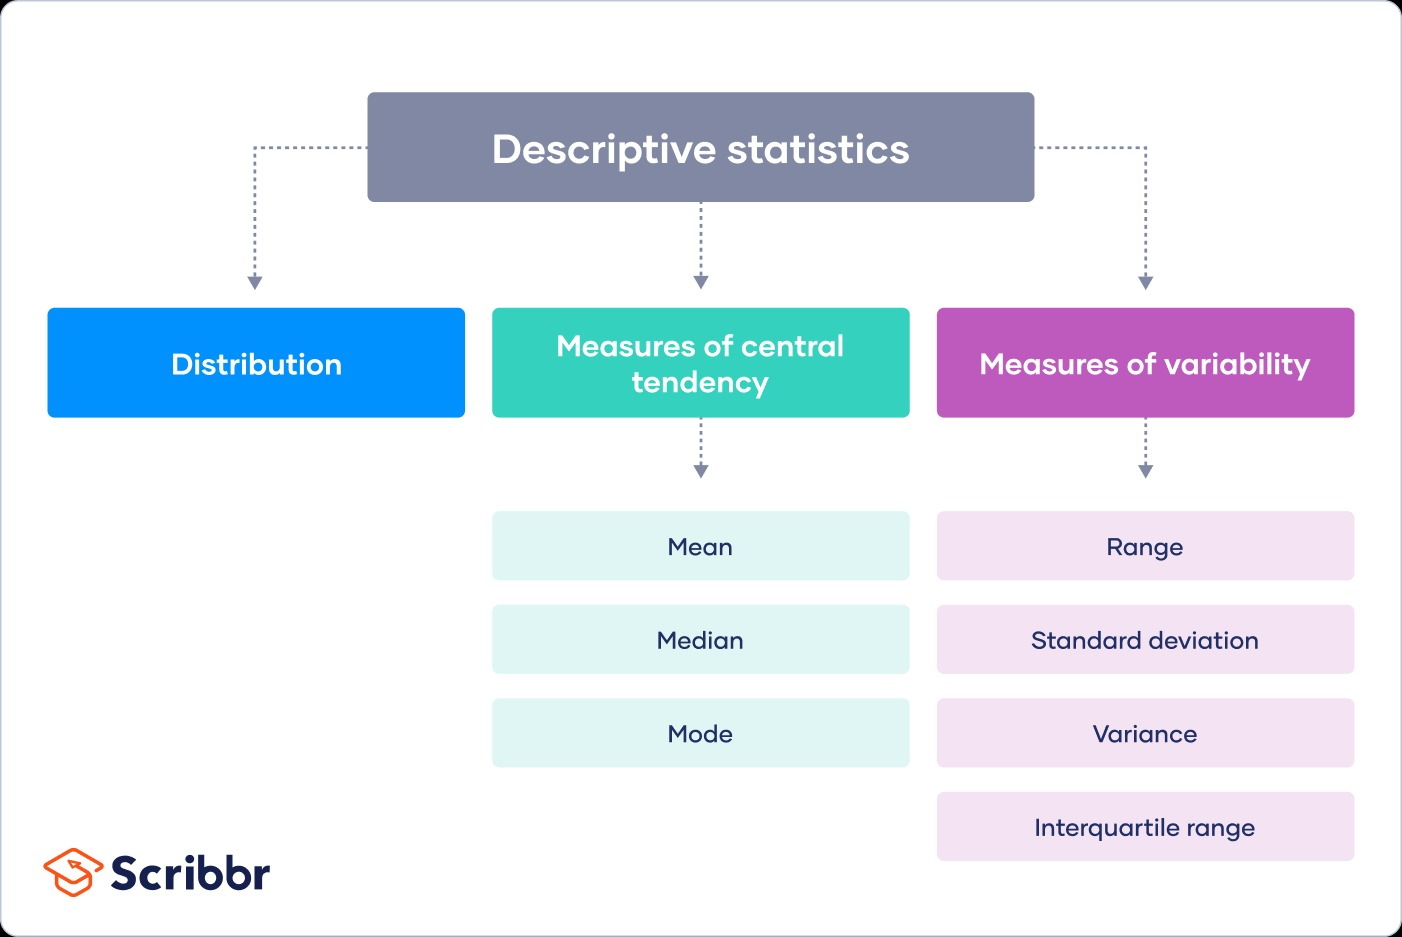
\includegraphics[width=1\textwidth,height=\textheight]{images/desc_stats.jpg}}

\hypertarget{distribution-1}{%
\subsection*{Distribution}\label{distribution-1}}
\addcontentsline{toc}{subsection}{Distribution}

fill

\hypertarget{simple}{%
\subsubsection*{Simple}\label{simple}}
\addcontentsline{toc}{subsubsection}{Simple}

fill

\hypertarget{grouped}{%
\subsubsection*{Grouped}\label{grouped}}
\addcontentsline{toc}{subsubsection}{Grouped}

fill

\hypertarget{central-tendency}{%
\subsection*{Central Tendency}\label{central-tendency}}
\addcontentsline{toc}{subsection}{Central Tendency}

fill

\hypertarget{mean}{%
\subsubsection*{Mean}\label{mean}}
\addcontentsline{toc}{subsubsection}{Mean}

fill

\hypertarget{median}{%
\subsubsection*{Median}\label{median}}
\addcontentsline{toc}{subsubsection}{Median}

fill

\hypertarget{mode}{%
\subsubsection*{Mode}\label{mode}}
\addcontentsline{toc}{subsubsection}{Mode}

fill

\hypertarget{variability}{%
\subsection*{Variability}\label{variability}}
\addcontentsline{toc}{subsection}{Variability}

fill

Range Standard Deviation Variance

fill

\hypertarget{inferential-statistics}{%
\section{Inferential Statistics}\label{inferential-statistics}}

fill

\hypertarget{t-tests}{%
\subsection*{t-tests}\label{t-tests}}
\addcontentsline{toc}{subsection}{t-tests}

fill

\hypertarget{anovas}{%
\subsection*{ANOVAs}\label{anovas}}
\addcontentsline{toc}{subsection}{ANOVAs}

fill

\hypertarget{regressions}{%
\subsection*{Regressions}\label{regressions}}
\addcontentsline{toc}{subsection}{Regressions}

fill

\hypertarget{appendix}{%
\chapter{Appendix}\label{appendix}}

\hypertarget{assignments}{%
\section{Assignments}\label{assignments}}

\hypertarget{individual}{%
\subsection*{Individual}\label{individual}}
\addcontentsline{toc}{subsection}{Individual}

\hypertarget{welcome-post}{%
\subsubsection*{Welcome Post}\label{welcome-post}}
\addcontentsline{toc}{subsubsection}{Welcome Post}

Because this course has a final team project that requires a significant amount of work, it is best to get started early. To assist with this, the first assignment is a welcome post. Within this course on Blackboard, you must post a welcome post. In this welcome post, include an image of yourself and answers to the following questions.

\begin{enumerate}
\def\labelenumi{\arabic{enumi}.}
\tightlist
\item
  What is your name?
\item
  Where are you from?
\item
  What is your desired career?
\item
  What is your favorite hobby?
\item
  What is your biggest pet peeve?
\item
  What is your favorite media properties to consume (e.g., \emph{The West Wing,} \emph{One Punch Man}, \emph{Call of Duty}, \emph{Harry Potter})?
\item
  What would you like to study this semester? (\emph{this can be specific or broad})
\end{enumerate}

\hypertarget{irb-certification}{%
\subsubsection*{IRB Certification}\label{irb-certification}}
\addcontentsline{toc}{subsubsection}{IRB Certification}

Be sure to complete the~\href{https://www.citiprogram.org/Shibboleth.sso/Login?target=https\%3A\%2F\%2Fwww.citiprogram.org\%2FSecure\%2FWelcome.cfm?inst=551\&entityID=https\%3A\%2F\%2Fsts.windows.net\%2F99f37d21-0b5c-43ea-9103-e16f02f5aecf\%2F}{CITI training}.

\hypertarget{apa-assignment}{%
\subsubsection*{APA Assignment}\label{apa-assignment}}
\addcontentsline{toc}{subsubsection}{APA Assignment}

Please provide accurate APA Reference List citations for the references provided on Blackboard in a .docx file. Please submit as a .doc or .docx file. Be sure to follow APA 7th Edition rules.

\hypertarget{annotated-bibliography}{%
\subsubsection*{Annotated Bibliography}\label{annotated-bibliography}}
\addcontentsline{toc}{subsubsection}{Annotated Bibliography}

Individuals are tasked with submitting a set of four (4) annotated bibliographies that are potentially relevant to their paper. Individuals are to submit unique annotated bibliographies. This means that if you and your team members collaborate on finding sources, you each must annotate different sources.. I recommned at least being from an academic paper or reputible scholarly book (preference toward paper).

I will attach a word document with formatting and content suggestions to this assignment.

\hypertarget{visualization-assignment}{%
\subsubsection*{Visualization Assignment}\label{visualization-assignment}}
\addcontentsline{toc}{subsubsection}{Visualization Assignment}

The visualization assignment will be posted as an .Rmd file on Blackboard. You are expected to create a new R Project for this assignment and then submit the zipped project on Blackboard. You may work on this as a group; however, I expect your visualizations to be moderately unique. \textbf{Do not plagiarize!}

\hypertarget{analysis-assignment}{%
\subsubsection*{Analysis Assignment}\label{analysis-assignment}}
\addcontentsline{toc}{subsubsection}{Analysis Assignment}

The analysis assignment will be posted as an .Rmd file on Blackboard. You are expected to create a new R Project for this assignment and then submit the zipped project on Blackboard. Each analysis question will require the code to run the analysis and your individual interpretation. You may work on this as a group; however, I expect your interpretation to be in your own words. \textbf{Do not plagiarize!}

\hypertarget{section-quizzes}{%
\subsubsection*{Section Quizzes}\label{section-quizzes}}
\addcontentsline{toc}{subsubsection}{Section Quizzes}

I will divide your book into five (5) sections and create five (5) minor quizzes. These quizzes will be posted around midterm. You will then have until the last week of class (before final's week) to submit all the quizzes.

\hypertarget{team}{%
\subsection*{Team}\label{team}}
\addcontentsline{toc}{subsection}{Team}

\hypertarget{partner-contract}{%
\subsubsection*{Partner Contract}\label{partner-contract}}
\addcontentsline{toc}{subsubsection}{Partner Contract}

I will attach a word document on Blackboard as a template partner contract. All team members must sign before submission.

\textbf{Common Tasks (\emph{suggestions)}\\
}Outliner\\
Reference Manager\\
Run analyses (in R)\\
Create visualizations (in R)\\
Reference Summarizer\\
Presenter\\
Lead Writer for Section (\href{https://psychology.ucsd.edu/_files/undergrad/writingresearchpapersinapastyleguide.pdf}{How to Write APA Style Research Papers})

\begin{enumerate}
\def\labelenumi{\arabic{enumi}.}
\item
  Introduction
\item
  Literature Review
\item
  Methodology
\item
  Results
\item
  Discussion
\item
  Conclusion
\end{enumerate}

\hypertarget{topic-selection}{%
\subsubsection*{Topic Selection}\label{topic-selection}}
\addcontentsline{toc}{subsubsection}{Topic Selection}

Submit your topic selection, including potential theories and rough research hypotheses or questions.

You can find theories in the theories chapter.

\emph{\textbf{Example}: We plan to survey students to identify a correlation between media usage and satisfaction. Borrowing from uses and gratification theory (though our theory choice may change as we spend more time reading), we expect individuals to select their media based upon the needs they are attempting to fulfill. Types of media include traditional (e.g., television, movies) and new (e.g., TikTok, YouTube). We are interested in if any usage impacts quality of life and if quantity of usage controls for some variation. If we receive a diverse enough participant pool, we are also interested in home type (i.e., single, family {[}as child{]}, friends, partner, family {[}as parent{]}). Our interest in home type is a reflection of the pandemic's limiting of outside interaction.}

\hypertarget{irb-application}{%
\subsubsection*{IRB Application}\label{irb-application}}
\addcontentsline{toc}{subsubsection}{IRB Application}

Each student must submit proof of IRB application submission. Each team \textbf{must} add me to their application so that I can access the material. You are graded on submitting a full application on time and how few revisions are required to pass. \ul{\textbf{Please reach out to me before}} submission so I can advise you on your project and accuracy.

\hypertarget{research-questionshypotheses}{%
\subsubsection*{Research Questions/Hypotheses}\label{research-questionshypotheses}}
\addcontentsline{toc}{subsubsection}{Research Questions/Hypotheses}

You are to present at least two (2) \textbf{concise} research questions (RQ) or hypotheses (RH) that your team want to examine. These RQs/RHs must include at least one (1) independent variable and one (1) dependent variable. These variables must be measurable for your project. If you have questions, please reach out before this assignment is due.

\hypertarget{research-proposal}{%
\subsubsection*{Research Proposal}\label{research-proposal}}
\addcontentsline{toc}{subsubsection}{Research Proposal}

Your research proposal is intended to be your first three (3) sections of your research paper: literature review, research objective, and methods. The proposal does not have to be a perfect version of these sections; however, the closer these are to complete, the work your team will have later in the semester.

I will post more specifics on Blackboard during the semester.

\hypertarget{outline}{%
\subsubsection*{Outline}\label{outline}}
\addcontentsline{toc}{subsubsection}{Outline}

Your outline is intended to give me a sneak peak of where you stand with your final three (3) sections of your research paper (i.e., results, discussion, and conclusion) before your final paper is due. The outline must be in numbers/bulleted format and not paragraph. The text in the outline can either be small phrases or full sentences. This is your final chance for feedback before you focus down on your final project.

\hypertarget{full-paper}{%
\subsubsection*{Full Paper}\label{full-paper}}
\addcontentsline{toc}{subsubsection}{Full Paper}

At the completion of this course, all student will have to submit a full research paper with their teams. Specifics will be presented throughout the semester.

\hypertarget{presentation}{%
\subsubsection*{Presentation}\label{presentation}}
\addcontentsline{toc}{subsubsection}{Presentation}

To accompany your final paper, your group is required to present your paper. Not all members have to present; however, this relies on your partner contract.

The presentation will be done during our scheduled time for our final (December 12, 10-11:40 am).~

\begin{itemize}
\item
  7-10 minutes
\item
  Powerpoint
\item
  Include key sections (Literature, RQ/RH, Methods, Results, Discussion)
\item
  Provide context
\end{itemize}

Beyond that, your presentation is up to you.

Submit your PowerPoint slides on Blackboard. You must also submit your partner contract with any important changes and commentary to reflect an imbalance in workload.

  \bibliography{book.bib,packages.bib}

\end{document}
